\documentclass[a4paper,12pt]{article}

\usepackage[utf8]{inputenc}
\usepackage{amsmath}
\usepackage{graphicx}
\usepackage{float}
\usepackage{hyperref}
\usepackage{ragged2e}
\title{Relatório sobre Conjuntos, Funções e Operadores Fuzzy}
\author{Doutorado CEFET}
\date{\today}

\begin{document}

\maketitle
\justifying
\section{Introdução}
Este relatório apresenta a implementação e análise de funções de pertinência, fuzzificação, operações fuzzy e relações fuzzy. As funções de pertinência são amplamente utilizadas em lógica fuzzy para representar graus de pertencimento de elementos a conjuntos fuzzy.

\section{Funções de Pertinência}
\subsection{Implementação de Funções de Pertinência}

As funções de pertinência implementadas incluem:


As funções de pertinência implementadas incluem as formas Triangular, Trapezoidal, Gaussiana, Sigmoidal, Sinoidal (Bell), Função S, Função Z, Cauchy, Gaussiana Dupla, Logarítmica e Retangular. Cada uma dessas funções possui características específicas que as tornam adequadas para diferentes aplicações em lógica fuzzy, permitindo modelar graus de pertinência de forma contínua e adaptável às necessidades do sistema.

Para a construção dos gráficos utilizando Python, utilizamos a função $plot_results$
    
\subsubsection{Função Triangular}
A função triangular é definida por três parâmetros $(a, b, c)$, onde:
\begin{itemize}
    \item $a$ é o ponto inicial onde a pertinência começa a aumentar;
    \item $b$ é o ponto onde a pertinência atinge o valor máximo (1);
    \item $c$ é o ponto final onde a pertinência retorna a 0.
\end{itemize}
A fórmula é dada por:
\[
\mu(x) =
\begin{cases}
\frac{x - a}{b - a}, & \text{se } a \leq x < b, \\
\frac{c - x}{c - b}, & \text{se } b \leq x < c, \\
0, & \text{caso contrário.}
\end{cases}
\]

\begin{figure}[H]
    \centering
    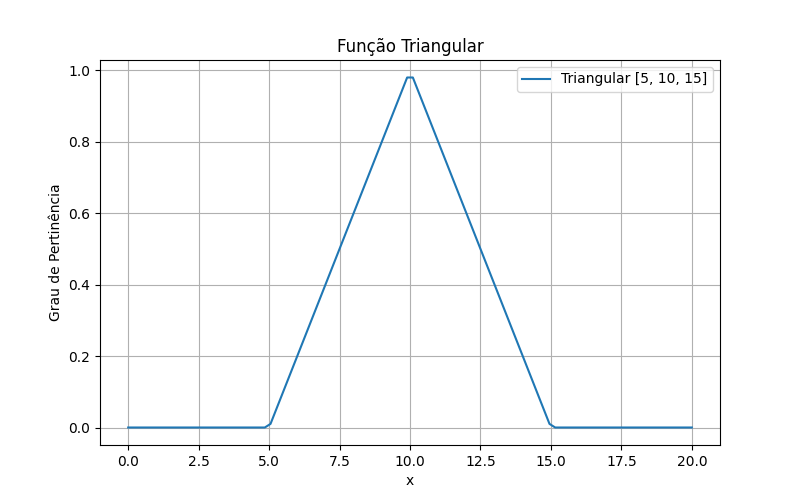
\includegraphics[width=0.8\textwidth]{img/triangular.png}
    \caption{Exemplo de função triangular com $a=5$, $b=10$, $c=15$.}
    \label{fig:funcao_triangular}
\end{figure}

\subsubsection{Função Trapezoidal}
A função trapezoidal é definida por quatro parâmetros $(a, b, c, d)$, onde:
\begin{itemize}
    \item $a$ e $d$ são os pontos onde a pertinência é 0;
    \item $b$ e $c$ definem a região onde a pertinência é 1.
\end{itemize}
A fórmula é:
\[
\mu(x) =
\begin{cases}
\frac{x - a}{b - a}, & \text{se } a \leq x < b, \\
1, & \text{se } b \leq x \leq c, \\
\frac{d - x}{d - c}, & \text{se } c < x \leq d, \\
0, & \text{caso contrário.}
\end{cases}
\]
\begin{figure}[H]
    \centering
    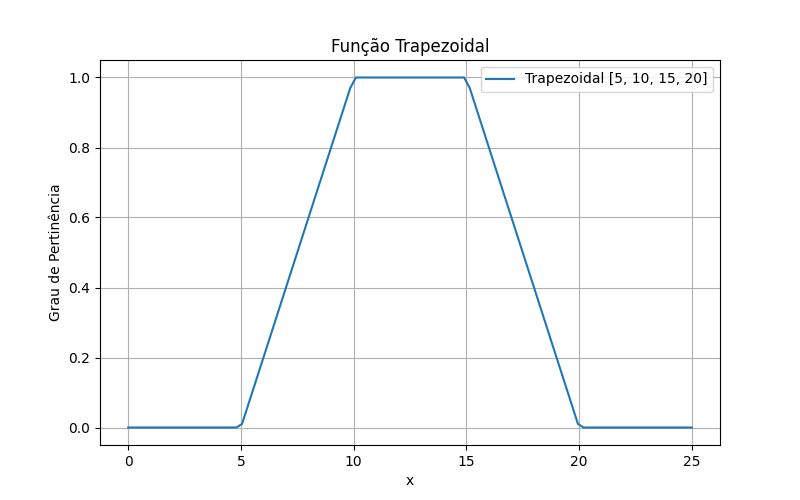
\includegraphics[width=0.8\textwidth]{img/trapezoidal.png}
    \caption{Exemplo de função trapezoidal com $a=5$, $b=10$, $c=15$, $d=20$.}
    \label{fig:funcao_trapezoidal}
\end{figure}

\subsubsection{Função Gaussiana}
A função gaussiana é definida por dois parâmetros $(c, \sigma)$, onde:
\begin{itemize}
    \item $c$ é o centro da curva, onde a pertinência é máxima (1);
    \item $\sigma$ controla a largura da curva.
\end{itemize}
A fórmula é:
\[
\mu(x) = e^{-\frac{1}{2} \left( \frac{x - c}{\sigma} \right)^2}.
\]
\begin{figure}[H]
    \centering
    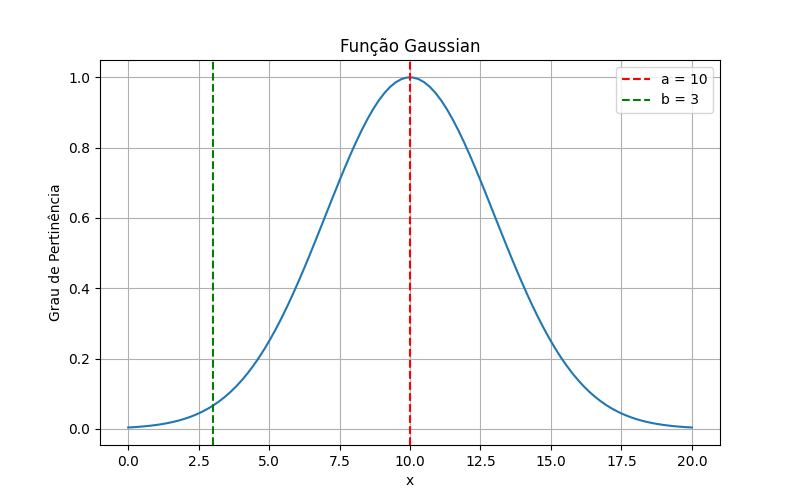
\includegraphics[width=0.8\textwidth]{img/gaussian.png}
    \caption{Exemplo de função gaussiana com $c=10$, $\sigma=3$.}
    \label{fig:funcao_gaussiana}
\end{figure}

\subsubsection{Função Sigmoidal}
A função sigmoidal é definida por dois parâmetros $(a, c)$, onde:
\begin{itemize}
    \item $a$ controla a inclinação da curva;
    \item $c$ é o ponto central onde a pertinência é 0.5.
\end{itemize}
A fórmula é:
\[
\mu(x) = \frac{1}{1 + e^{-a(x - c)}}.
\]

\begin{figure}[H]
    \centering
    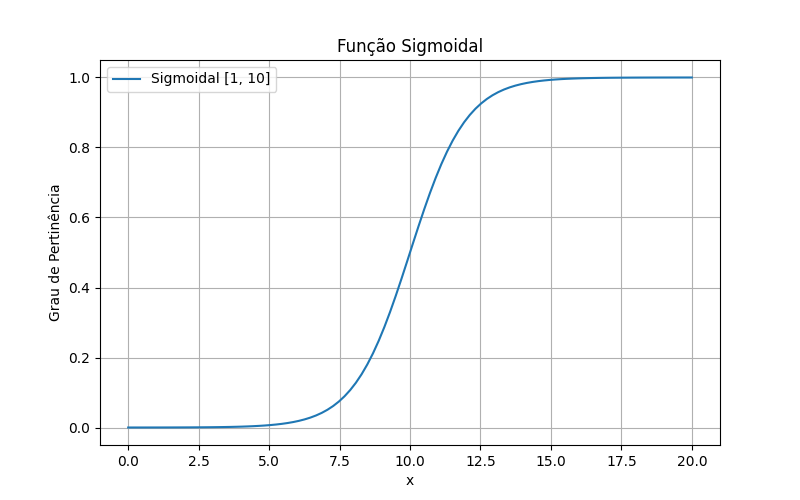
\includegraphics[width=0.8\textwidth]{img/sigmoidal.png}
    \caption{Exemplo de função sigmoidal com $a=1$, $c=10$.}
    \label{fig:funcao_sigmoidal}
\end{figure}

\subsubsection{Função Sinoidal (Bell)}
A função Bell é definida por três parâmetros $(a, b, c)$, onde:
\begin{itemize}
    \item $a$ controla a largura da curva;
    \item $b$ controla a inclinação;
    \item $c$ é o centro da curva.
\end{itemize}
A fórmula é:
\[
\mu(x) = \frac{1}{1 + \left|\frac{x - c}{a}\right|^{2b}}.
\]
\begin{figure}[H]
    \centering
    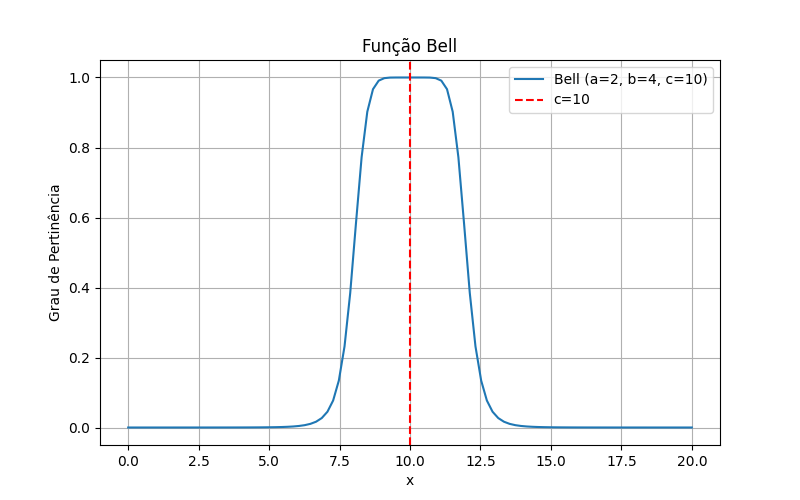
\includegraphics[width=0.8\textwidth]{img/bell.png}
    \caption{Exemplo de função Bell com $a=2$, $b=4$, $c=10$.}
    \label{fig:funcao_bell}
\end{figure}

\subsubsection{Função S}
A função S é definida por dois parâmetros $(a, b)$, onde:
\begin{itemize}
    \item $a$ é o ponto onde a pertinência começa a aumentar;
    \item $b$ é o ponto onde a pertinência atinge 1.
\end{itemize}
A fórmula é:
\[
\mu(x) =
\begin{cases}
0, & \text{se } x \leq a, \\
2\left(\frac{x - a}{b - a}\right)^2, & \text{se } a < x < b, \\
1, & \text{se } x \geq b.
\end{cases}
\]
\begin{figure}[H]
    \centering
    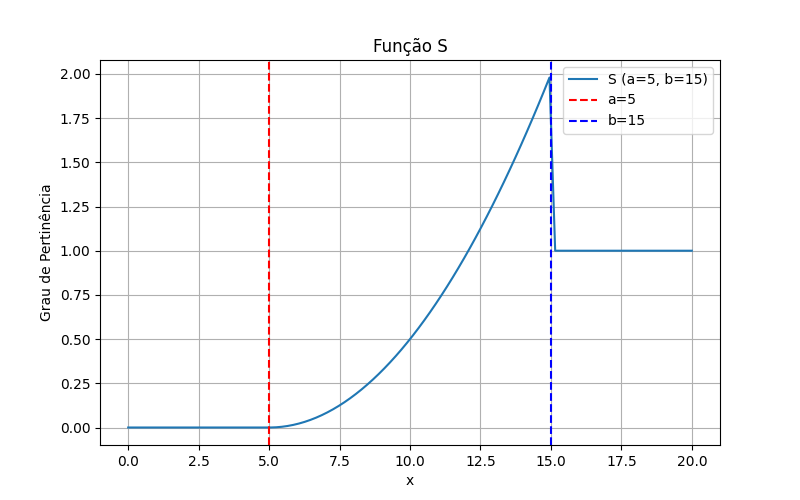
\includegraphics[width=0.8\textwidth]{img/s.png}
    \caption{Exemplo de função S com $a=5$, $b=15$.}
    \label{fig:funcao_s}
\end{figure}

\subsubsection{Função Z}
A função Z é definida por dois parâmetros $(a, b)$, onde:
\begin{itemize}
    \item $a$ é o ponto onde a pertinência começa a diminuir;
    \item $b$ é o ponto onde a pertinência atinge 0.
\end{itemize}
A fórmula é:
\[
\mu(x) =
\begin{cases}
1, & \text{se } x \leq a, \\
1 - 2\left(\frac{x - a}{b - a}\right)^2, & \text{se } a < x < b, \\
0, & \text{se } x \geq b.
\end{cases}
\]

\begin{figure}[H]
    \centering
    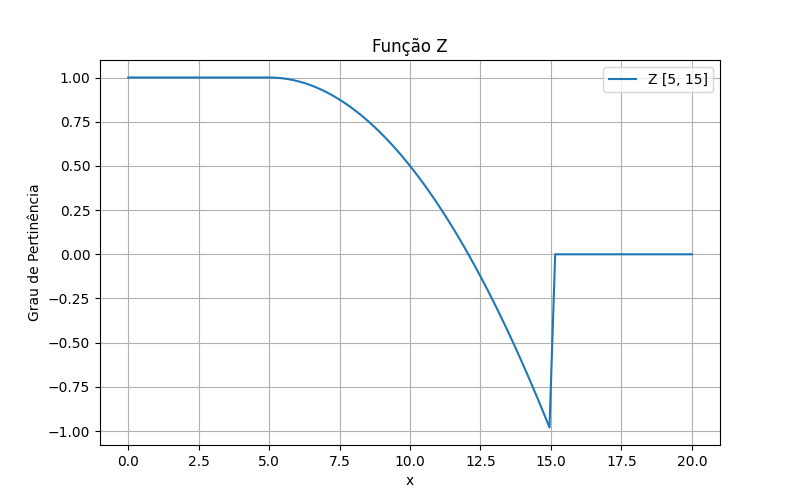
\includegraphics[width=0.8\textwidth]{img/z.png}
    \caption{Exemplo de função Z com $a=5$, $b=15$.}
    \label{fig:funcao_z}
\end{figure}

\subsubsection{Função Cauchy}
A função Cauchy é definida por dois parâmetros $(c, \gamma)$, onde:
\begin{itemize}
    \item $c$ é o centro da curva;
    \item $\gamma$ controla a largura da curva.
\end{itemize}
A fórmula é:
\[
\mu(x) = \frac{1}{1 + \left(\frac{x - c}{\gamma}\right)^2}.
\]
\begin{figure}[H]
    \centering
    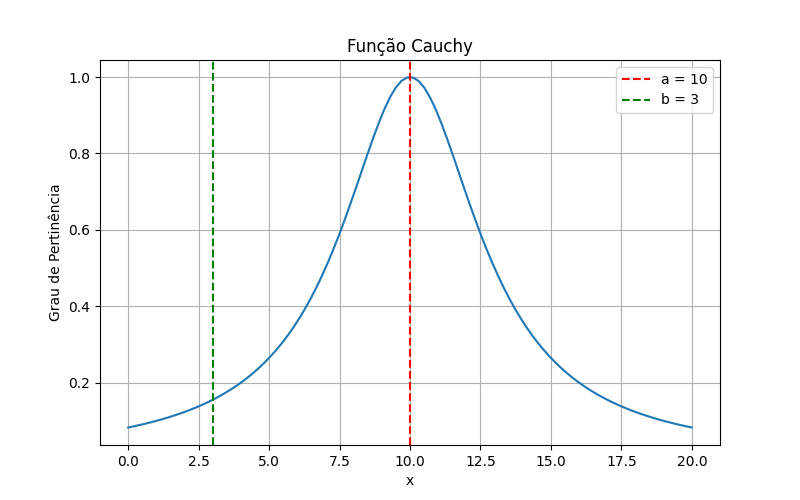
\includegraphics[width=0.8\textwidth]{img/cauchy.png}
    \caption{Exemplo de função Cauchy com $c=10$, $\gamma=3$.}
    \label{fig:funcao_cauchy}
\end{figure}

\subsubsection{Função Gaussiana Dupla}
A função Gaussiana Dupla é definida por três parâmetros $(c, \sigma_1, \sigma_2)$, onde:
\begin{itemize}
    \item $c$ é o centro da curva;
    \item $\sigma_1$ controla a largura da curva para $x \leq c$;
    \item $\sigma_2$ controla a largura da curva para $x > c$.
\end{itemize}
A fórmula é:
\[
\mu(x) =
\begin{cases}
e^{-\frac{1}{2} \left( \frac{x - c}{\sigma_1} \right)^2}, & \text{se } x \leq c, \\
e^{-\frac{1}{2} \left( \frac{x - c}{\sigma_2} \right)^2}, & \text{se } x > c.
\end{cases}
\]
\begin{figure}[H]
    \centering
    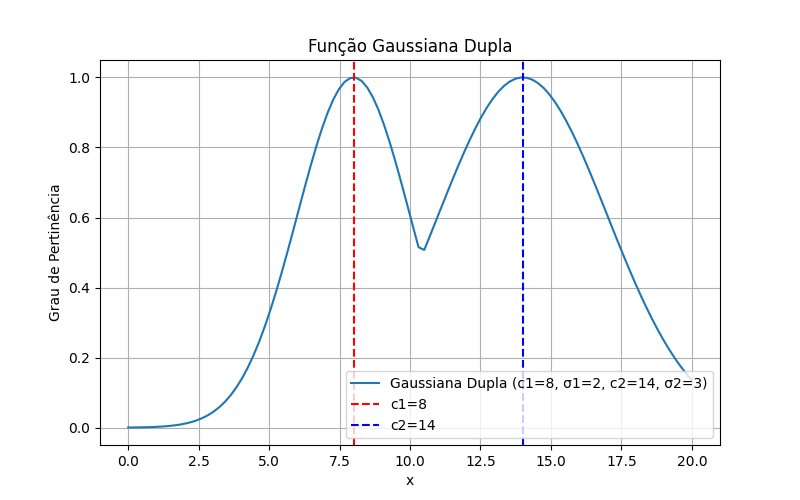
\includegraphics[width=0.8\textwidth]{img/double_gaussian.png}
    \caption{Exemplo de função Gaussiana Dupla com $c=10$, $\sigma_1=3$, $\sigma_2=5$.}
    \label{fig:funcao_gaussiana_dupla}
\end{figure}

\subsubsection{Função Retangular}
A função Retangular é definida por dois parâmetros $(a, b)$, onde:
\begin{itemize}
    \item $a$ é o início do intervalo onde a pertinência é 1;
    \item $b$ é o final do intervalo onde a pertinência é 1.
\end{itemize}
A fórmula é:
\[
\mu(x) =
\begin{cases}
1, & \text{se } a \leq x \leq b, \\
0, & \text{caso contrário.}
\end{cases}
\]
\begin{figure}[H]
    \centering
    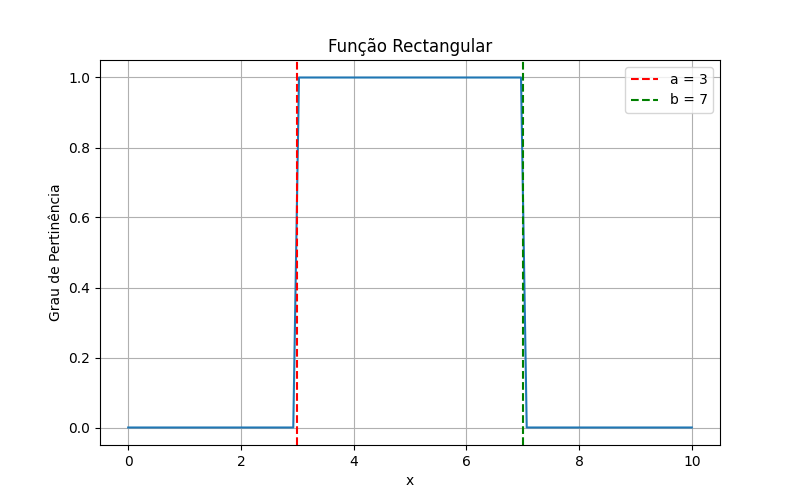
\includegraphics[width=0.8\textwidth]{img/rectangular.png}
    \caption{Exemplo de função Retangular com $a=10$, $b=20$.}
    \label{fig:funcao_retangular}
\end{figure}

\subsubsection{Função Logarítmica}
A função Logarítmica é definida por dois parâmetros $(a, b)$, onde:
\begin{itemize}
    \item $a$ controla o deslocamento da curva;
    \item $b$ controla a inclinação da curva.
\end{itemize}
A fórmula é:
\[
\mu(x) = 
\begin{cases}
0, & \text{se } x \leq a, \\
\log_b(x - a + 1), & \text{se } x > a.
\end{cases}
\]
\begin{figure}[H]
    \centering
    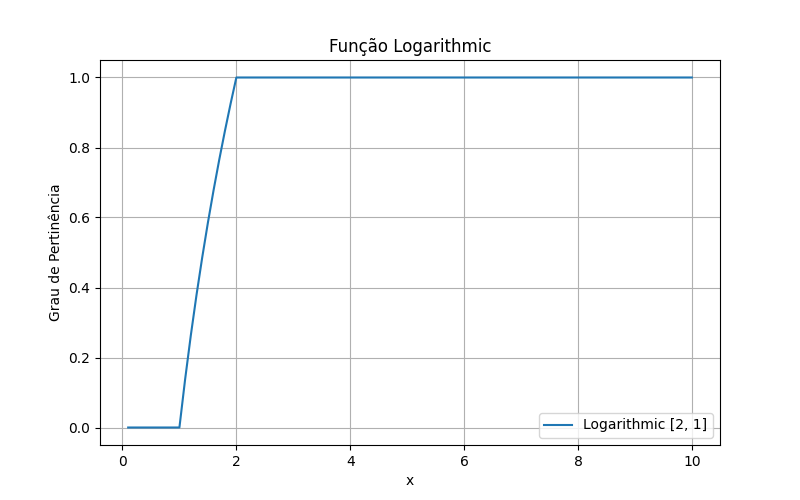
\includegraphics[width=0.8\textwidth]{img/logarithmic.png}
    \caption{Exemplo de função Logarítmica com $a=5$, $b=2$.}
    \label{fig:funcao_logaritmica}
\end{figure}


\subsection{Fuzzificação e Análise Comparativa}

Para a fuzzificação, escolhemos uma variável de entrada com universo de discurso definido e particionamos o domínio em funções de pertinência uniformemente espaçadas. A seguir, apresentamos os resultados para duas amostras distintas.

Para as variáveis de entrada, definimos um universo de estudo como segue, particionando esse domínio em cinco funções de pertinência uniformemente espaçadas:

\begin{table}[H]
\centering
\caption{Categorias de Temperatura e Intervalos}
\label{tab:categorias_temperatura}
\begin{tabular}{|c|c|}
\hline
\textbf{Categoria}    & \textbf{Intervalo de Temperatura (°C)} \\ \hline
Muito Frio            & $0$ a $20$                            \\ \hline
Frio                  & $20$ a $40$                           \\ \hline
Morno                 & $40$ a $60$                           \\ \hline
Quente                & $60$ a $80$                           \\ \hline
Muito Quente          & $80$ a $100$                          \\ \hline
\end{tabular}
\end{table}

\subsubsection{Fuzzificação com Funções Triangulares}

Para a variável linguística \textbf{Temperatura}, foram definidos cinco conjuntos fuzzy com os seguintes intervalos e parâmetros, além das ativações calculadas para as amostras \textbf{25} e \textbf{75}:

\begin{table}[H]
\centering
\caption{Conjuntos Fuzzy, Intervalos, Parâmetros e Ativações}
\begin{tabular}{|c|c|c|c|}
\hline
\textbf{Categoria}    & \textbf{Intervalo (°C)} & \textbf{Parâmetros}       & \textbf{Ativações [25, 75]} \\ \hline
Muita Fria            & $[0.0, 20.0]$          & $[0.0, 0.0, 25.0]$        & $[0, 0]$                   \\ \hline
Fria                  & $[20.0, 40.0]$         & $[0.0, 25.0, 50.0]$       & $[0.99, 0.0]$              \\ \hline
Morno                 & $[40.0, 60.0]$         & $[25.0, 50.0, 75.0]$      & $[0.01, 0.01]$             \\ \hline
Quente                & $[60.0, 80.0]$         & $[50.0, 75.0, 100.0]$     & $[0.0, 0.99]$              \\ \hline
Muito Quente          & $[80.0, 100.0]$        & $[75.0, 100.0, 100.0]$    & $[0, 0]$                   \\ \hline
\end{tabular}
\end{table}

A seguir, apresentamos o gráfico das funções de pertinência triangulares e suas ativações:

\begin{figure}[H]
    \centering
    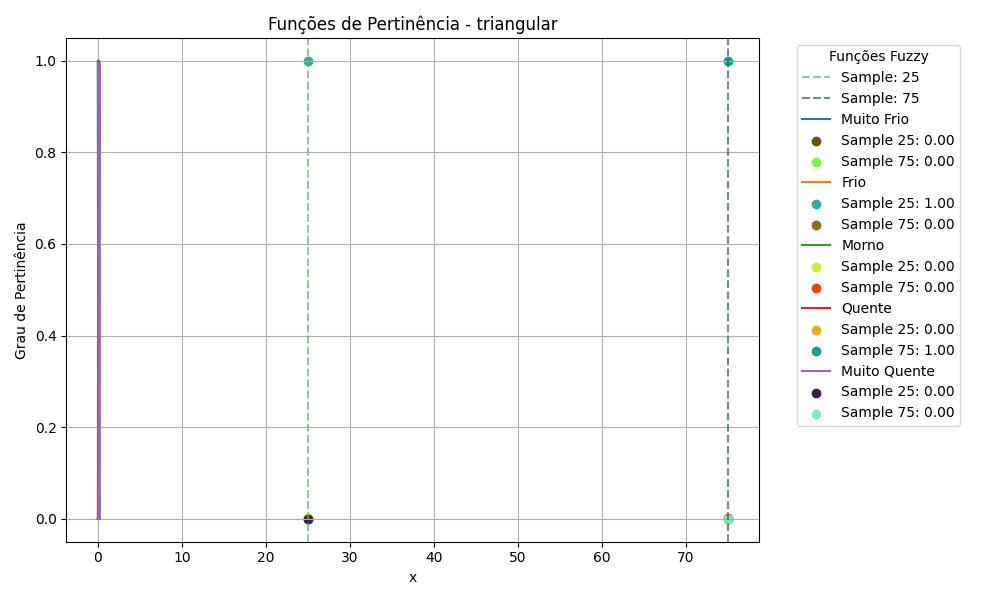
\includegraphics[width=0.8\textwidth]{img/funções_de_pertinência_triangular_fuzzificado.png}
    \caption{Funções de Pertinência Triangulares para a variável \textbf{Temperatura}.}
\end{figure}


\subsubsection{Fuzzificação com Funções Trapezoidais}

Para a variável linguística \textbf{Temperatura}, foram definidos cinco conjuntos fuzzy com os seguintes intervalos e parâmetros, além das ativações calculadas para as amostras \textbf{25} e \textbf{75}:

\begin{table}[H]
\centering
\caption{Conjuntos Fuzzy, Intervalos, Parâmetros e Ativações}
\begin{tabular}{|c|c|c|c|}
\hline
\textbf{Categoria}    & \textbf{Intervalo (°C)} & \textbf{Parâmetros}               & \textbf{Ativações [25, 75]} \\ \hline
Muita Fria            & $[0.0, 20.0]$          & $[0.0, 0.0, 12.5, 25.0]$         & $[0, 0]$                   \\ \hline
Fria                  & $[20.0, 40.0]$         & $[0.0, 12.5, 37.5, 50.0]$        & $[1, 0]$                   \\ \hline
Morno                 & $[40.0, 60.0]$         & $[25.0, 37.5, 62.5, 75.0]$       & $[0.02, 0.02]$             \\ \hline
Quente                & $[60.0, 80.0]$         & $[50.0, 62.5, 87.5, 100.0]$      & $[0, 1]$                   \\ \hline
Muito Quente          & $[80.0, 100.0]$        & $[75.0, 87.5, 100.0, 100.0]$     & $[0, 0]$                   \\ \hline
\end{tabular}
\end{table}

A seguir, apresentamos o gráfico das funções de pertinência trapezoidais e suas ativações:

\begin{figure}[H]
    \centering
    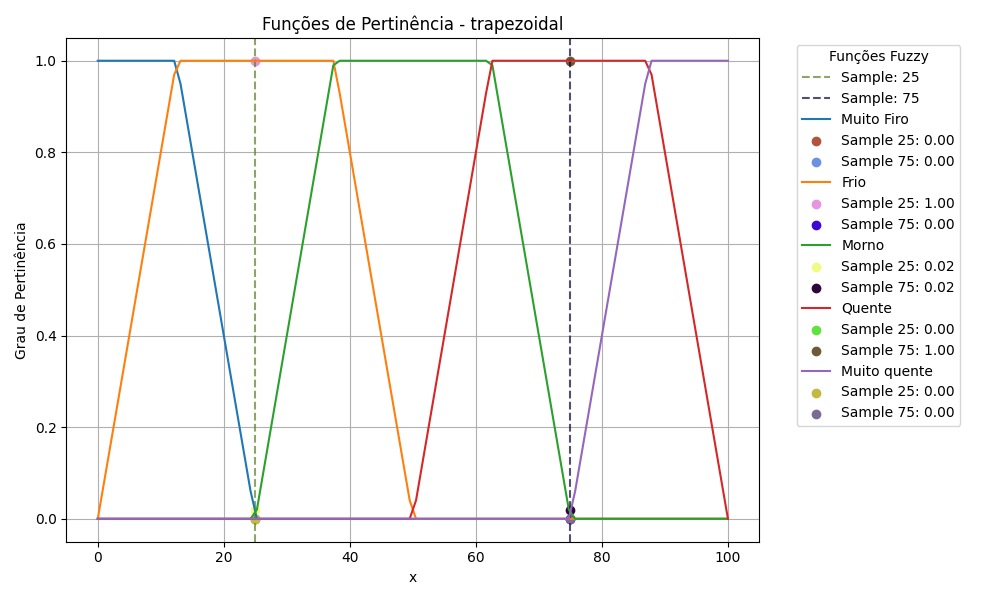
\includegraphics[width=0.8\textwidth]{img/funções_de_pertinência_trapezoidal_fuzzificado.png}
    \caption{Funções de Pertinência Trapezoidais para a variável \textbf{Temperatura}.}
\end{figure}


\subsubsection{Fuzzificação com Funções Gaussianas}

Para a variável linguística \textbf{Temperatura}, foram definidos cinco conjuntos fuzzy com os seguintes intervalos e parâmetros, além das ativações calculadas para as amostras \textbf{25} e \textbf{75}:

\begin{table}[H]
\centering
\caption{Conjuntos Fuzzy, Intervalos, Parâmetros e Ativações}
\begin{tabular}{|c|c|c|c|}
\hline
\textbf{Categoria}    & \textbf{Intervalo (°C)} & \textbf{Parâmetros}       & \textbf{Ativações [25, 75]} \\ \hline
Muita Fria            & $[0.0, 20.0]$          & $[0.0, 12.5]$             & $[0.13, 0.0]$              \\ \hline
Fria                  & $[20.0, 40.0]$         & $[25.0, 12.5]$            & $[1.0, 0.0]$               \\ \hline
Morno                 & $[40.0, 60.0]$         & $[50.0, 12.5]$            & $[0.14, 0.14]$             \\ \hline
Quente                & $[60.0, 80.0]$         & $[75.0, 12.5]$            & $[0.0, 1.0]$               \\ \hline
Muito Quente          & $[80.0, 100.0]$        & $[100.0, 12.5]$           & $[0.0, 0.13]$              \\ \hline
\end{tabular}
\end{table}

A seguir, apresentamos o gráfico das funções de pertinência gaussianas e suas ativações:

\begin{figure}[H]
    \centering
    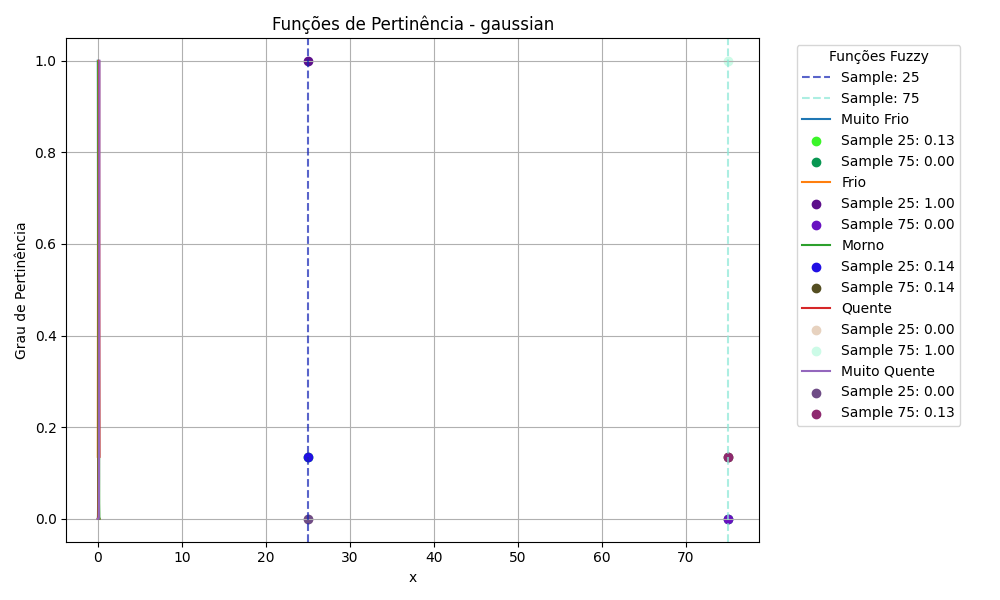
\includegraphics[width=0.8\textwidth]{img/funções_de_pertinência_gaussian_fuzzificado.png}
    \caption{Funções de Pertinência Gaussianas para a variável \textbf{Temperatura}.}
\end{figure}

\subsubsection{Fuzzificação com Funções Sigmoidais}

Para a variável linguística \textbf{Temperatura}, foram definidos cinco conjuntos fuzzy com os seguintes intervalos e parâmetros, além das ativações calculadas para as amostras \textbf{25} e \textbf{75}:

\begin{table}[H]
\centering
\caption{Conjuntos Fuzzy, Intervalos, Parâmetros e Ativações}
\begin{tabular}{|c|c|c|c|}
\hline
\textbf{Categoria}    & \textbf{Intervalo (°C)} & \textbf{Parâmetros}       & \textbf{Ativações [25, 75]} \\ \hline
Muita Fria            & $[0.0, 20.0]$          & $[1.0, 0.0]$              & $[1.0, 1.0]$               \\ \hline
Fria                  & $[20.0, 40.0]$         & $[1.0, 25.0]$             & $[0.56, 1.0]$             \\ \hline
Morno                 & $[40.0, 60.0]$         & $[1.0, 50.0]$             & $[0.0, 1.0]$              \\ \hline
Quente                & $[60.0, 80.0]$         & $[1.0, 75.0]$             & $[0.0, 0.44]$             \\ \hline
Muito Quente          & $[80.0, 100.0]$        & $[1.0, 100.0]$            & $[0.0, 0.0]$              \\ \hline
\end{tabular}
\end{table}

A seguir, apresentamos o gráfico das funções de pertinência sigmoidais e suas ativações:

\begin{figure}[H]
    \centering
    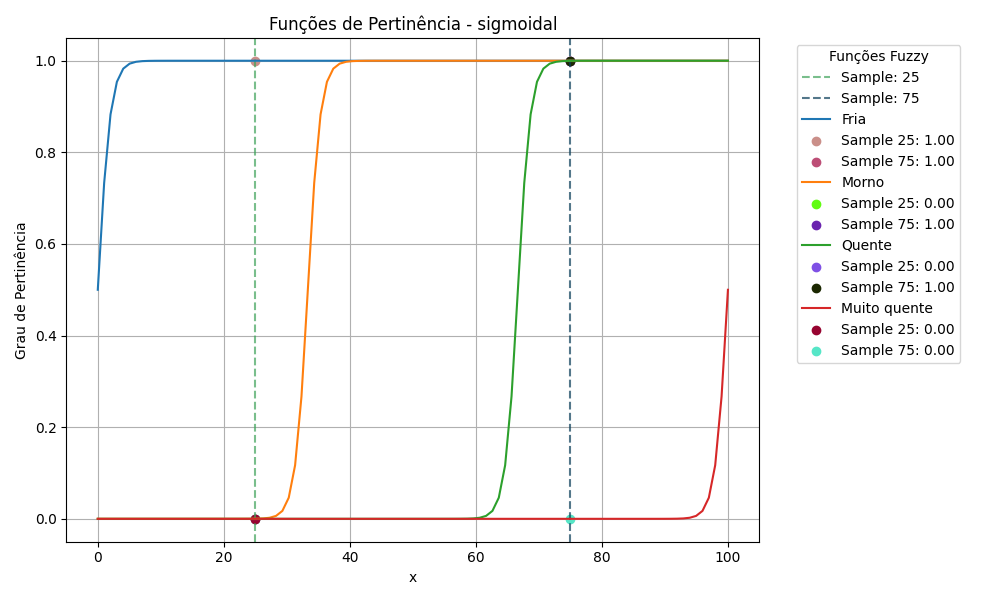
\includegraphics[width=0.8\textwidth]{img/funções_de_pertinência_sigmoidal_fuzzificado.png}
    \caption{Funções de Pertinência Sigmoidais para a variável \textbf{Temperatura}.}
\end{figure}

\subsubsection{Fuzzificação com Funções Bell}

Para a variável linguística \textbf{Temperatura}, foram definidos cinco conjuntos fuzzy com os seguintes intervalos e parâmetros, além das ativações calculadas para as amostras \textbf{25} e \textbf{75}:

\begin{table}[H]
\centering
\caption{Conjuntos Fuzzy, Intervalos, Parâmetros e Ativações}
\begin{tabular}{|c|c|c|c|}
\hline
\textbf{Categoria}    & \textbf{Intervalo (°C)} & \textbf{Parâmetros}       & \textbf{Ativações [25, 75]} \\ \hline
Muita Fria            & $[0.0, 20.0]$          & $[12.5, 2.0, 0.0]$        & $[0.06, 0.0]$              \\ \hline
Fria                  & $[20.0, 40.0]$         & $[12.5, 2.0, 25.0]$       & $[1.0, 0.0]$               \\ \hline
Morno                 & $[40.0, 60.0]$         & $[12.5, 2.0, 50.0]$       & $[0.06, 0.06]$             \\ \hline
Quente                & $[60.0, 80.0]$         & $[12.5, 2.0, 75.0]$       & $[0.0, 1.0]$               \\ \hline
Muito Quente          & $[80.0, 100.0]$        & $[12.5, 2.0, 100.0]$      & $[0.0, 0.06]$              \\ \hline
\end{tabular}
\end{table}

A seguir, apresentamos o gráfico das funções de pertinência Bell e suas ativações:

\begin{figure}[H]
    \centering
    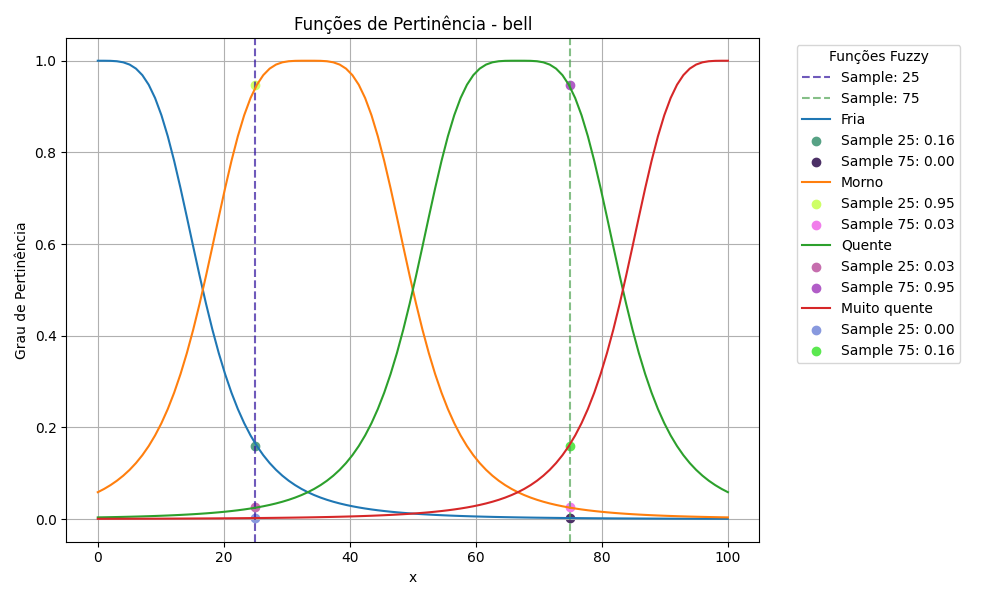
\includegraphics[width=0.8\textwidth]{img/funções_de_pertinência_bell_fuzzificado.png}
    \caption{Funções de Pertinência Bell para a variável \textbf{Temperatura}.}
\end{figure}

\subsubsection{Fuzzificação com Funções S}

Para a variável linguística \textbf{Temperatura}, foram definidos cinco conjuntos fuzzy com os seguintes intervalos e parâmetros, além das ativações calculadas para as amostras \textbf{25} e \textbf{75}:

\begin{table}[H]
\centering
\caption{Conjuntos Fuzzy, Intervalos, Parâmetros e Ativações}
\begin{tabular}{|c|c|c|c|}
\hline
\textbf{Categoria}    & \textbf{Intervalo (°C)} & \textbf{Parâmetros}       & \textbf{Ativações [25, 75]} \\ \hline
Muita Fria            & $[0.0, 20.0]$          & $[0.0, 25.0]$             & $[1, 1]$                   \\ \hline
Fria                  & $[20.0, 40.0]$         & $[25.0, 50.0]$            & $[0.0, 1.0]$               \\ \hline
Morno                 & $[40.0, 60.0]$         & $[50.0, 75.0]$            & $[0.0, 1.96]$              \\ \hline
Quente                & $[60.0, 80.0]$         & $[75.0, 100.0]$           & $[0, 0]$                   \\ \hline
Muito Quente          & $[80.0, 100.0]$        & $[100.0, 100.0]$          & $[0, 0]$                   \\ \hline
\end{tabular}
\end{table}

A seguir, apresentamos o gráfico das funções de pertinência S e suas ativações:

\begin{figure}[H]
    \centering
    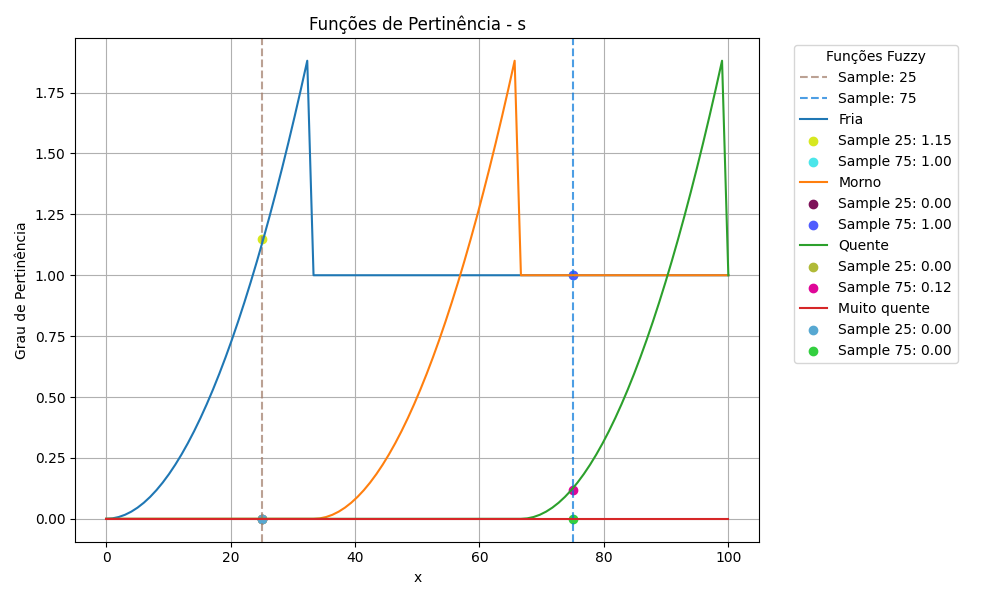
\includegraphics[width=0.8\textwidth]{img/funções_de_pertinência_s_fuzzificado.png}
    \caption{Funções de Pertinência S para a variável \textbf{Temperatura}.}
\end{figure}

\subsubsection{Fuzzificação com Funções Z}

Para a variável linguística \textbf{Temperatura}, foram definidos cinco conjuntos fuzzy com os seguintes intervalos e parâmetros, além das ativações calculadas para as amostras \textbf{25} e \textbf{75}:

\begin{table}[H]
\centering
\caption{Conjuntos Fuzzy, Intervalos, Parâmetros e Ativações}
\begin{tabular}{|c|c|c|c|}
\hline
\textbf{Categoria}    & \textbf{Intervalo (°C)} & \textbf{Parâmetros}       & \textbf{Ativações [25, 75]} \\ \hline
Muita Fria            & $[0.0, 20.0]$          & $[0.0, 0.0]$              & $[0, 0]$                   \\ \hline
Fria                  & $[20.0, 40.0]$         & $[0.0, 25.0]$             & $[0, 0]$                   \\ \hline
Morno                 & $[40.0, 60.0]$         & $[25.0, 50.0]$            & $[1.0, 0.0]$               \\ \hline
Quente                & $[60.0, 80.0]$         & $[50.0, 75.0]$            & $[1.0, -0.96]$             \\ \hline
Muito Quente          & $[80.0, 100.0]$        & $[75.0, 100.0]$           & $[1, 1]$                   \\ \hline
\end{tabular}
\end{table}

A seguir, apresentamos o gráfico das funções de pertinência Z e suas ativações:

\begin{figure}[H]
    \centering
    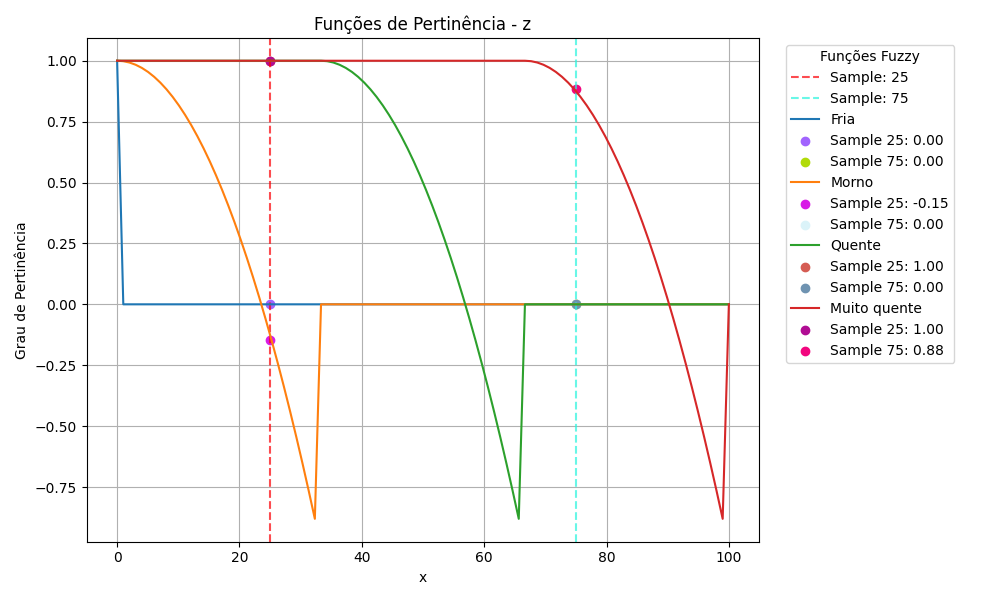
\includegraphics[width=0.8\textwidth]{img/funções_de_pertinência_z_fuzzificado.png}
    \caption{Funções de Pertinência Z para a variável \textbf{Temperatura}.}
\end{figure}

\subsubsection{Fuzzificação com Funções Pi}

Para a variável linguística \textbf{Temperatura}, foram definidos cinco conjuntos fuzzy com os seguintes intervalos e parâmetros, além das ativações calculadas para as amostras \textbf{25} e \textbf{75}:

\begin{table}[H]
\centering
\caption{Conjuntos Fuzzy, Intervalos, Parâmetros e Ativações}
\begin{tabular}{|c|c|c|c|}
\hline
\textbf{Categoria}    & \textbf{Intervalo (°C)} & \textbf{Parâmetros}       & \textbf{Ativações [25, 75]} \\ \hline
Muita Fria            & $[0.0, 20.0]$          & $[0.0, 0.0, 25.0]$        & $[0, 0]$                   \\ \hline
Fria                  & $[20.0, 40.0]$         & $[0.0, 25.0, 50.0]$       & $[1.0, 0.0]$               \\ \hline
Morno                 & $[40.0, 60.0]$         & $[25.0, 50.0, 75.0]$      & $[0.0, -0.96]$             \\ \hline
Quente                & $[60.0, 80.0]$         & $[50.0, 75.0, 100.0]$     & $[0.0, 1.96]$              \\ \hline
Muito Quente          & $[80.0, 100.0]$        & $[75.0, 100.0, 100.0]$    & $[0, 0]$                   \\ \hline
\end{tabular}
\end{table}

A seguir, apresentamos o gráfico das funções de pertinência Pi e suas ativações:

\begin{figure}[H]
    \centering
    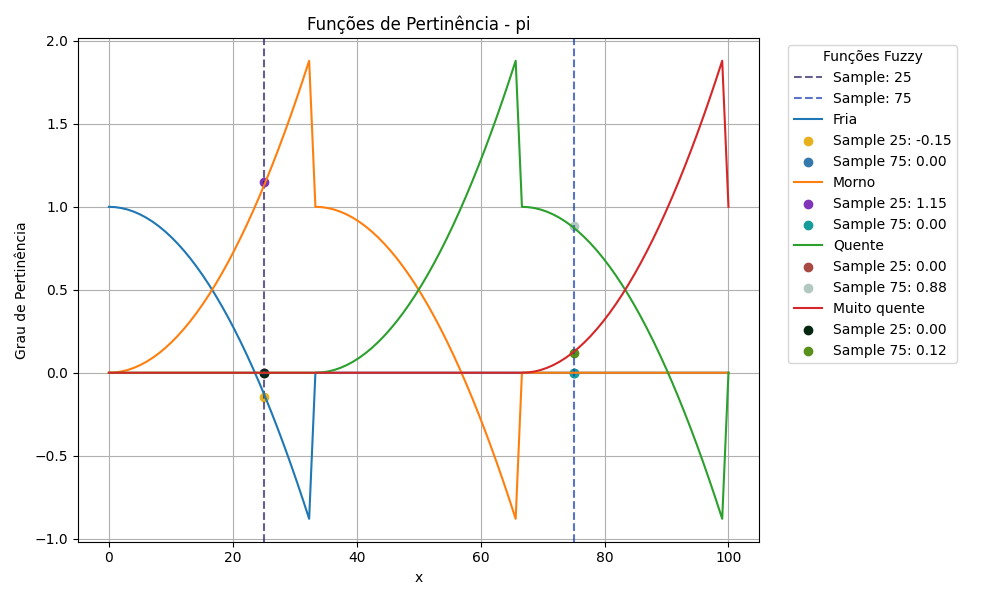
\includegraphics[width=0.8\textwidth]{img/funções_de_pertinência_pi_fuzzificado.png}
    \caption{Funções de Pertinência Pi para a variável \textbf{Temperatura}.}
\end{figure}

\subsubsection{Fuzzificação com Funções Singleton}

Para a variável linguística \textbf{Temperatura}, foram definidos cinco conjuntos fuzzy com os seguintes intervalos e parâmetros, além das ativações calculadas para as amostras \textbf{25} e \textbf{75}:

\begin{table}[H]
\centering
\caption{Conjuntos Fuzzy, Intervalos, Parâmetros e Ativações}
\begin{tabular}{|c|c|c|c|}
\hline
\textbf{Categoria}    & \textbf{Intervalo (°C)} & \textbf{Parâmetros}       & \textbf{Ativações [25, 75]} \\ \hline
Muita Fria            & $[0.0, 20.0]$          & $[0.0]$                   & $[0, 0]$                   \\ \hline
Fria                  & $[20.0, 40.0]$         & $[25.0]$                  & $[0, 0]$                   \\ \hline
Morno                 & $[40.0, 60.0]$         & $[50.0]$                  & $[0, 0]$                   \\ \hline
Quente                & $[60.0, 80.0]$         & $[75.0]$                  & $[0, 0]$                   \\ \hline
Muito Quente          & $[80.0, 100.0]$        & $[100.0]$                 & $[0, 0]$                   \\ \hline
\end{tabular}
\end{table}

A seguir, apresentamos o gráfico das funções de pertinência Singleton e suas ativações:

\begin{figure}[H]
    \centering
    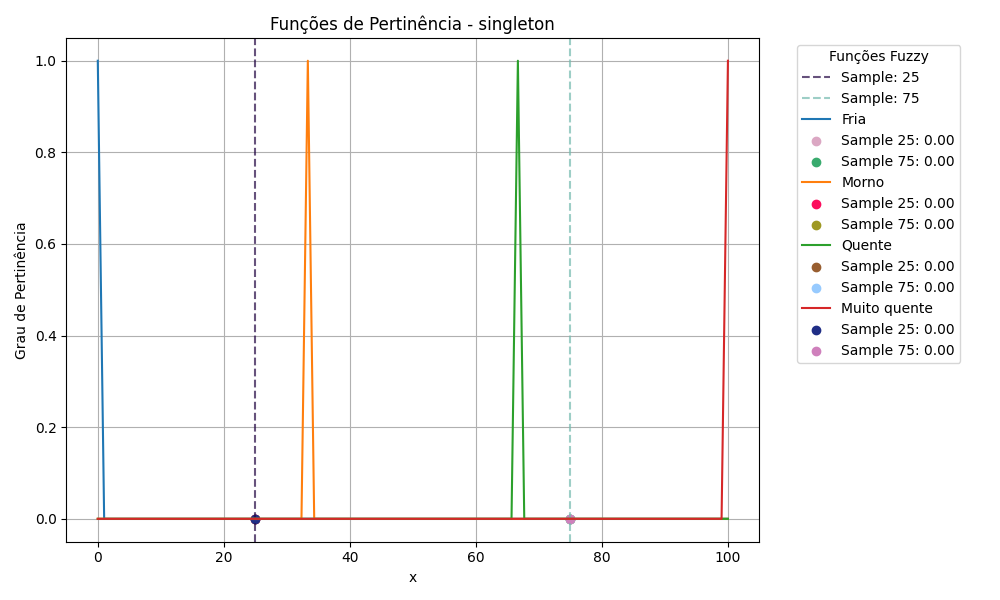
\includegraphics[width=0.8\textwidth]{img/funções_de_pertinência_singleton_fuzzificado.png}
    \caption{Funções de Pertinência Singleton para a variável \textbf{Temperatura}.}
\end{figure}
\subsubsection{Fuzzificação com Funções Cauchy}

Para a variável linguística \textbf{Temperatura}, foram definidos cinco conjuntos fuzzy com os seguintes intervalos e parâmetros, além das ativações calculadas para as amostras \textbf{25} e \textbf{75}:

\begin{table}[H]
\centering
\caption{Conjuntos Fuzzy, Intervalos, Parâmetros e Ativações (Cauchy)}
\begin{tabular}{|c|c|c|c|}
\hline
\textbf{Categoria}    & \textbf{Intervalo (°C)} & \textbf{Parâmetros}       & \textbf{Ativações [25, 75]} \\ \hline
Muita Fria            & $[0.0, 20.0]$          & $[0.0, 12.5]$             & $[0.2, 0.03]$              \\ \hline
Fria                  & $[20.0, 40.0]$         & $[25.0, 12.5]$            & $[1.0, 0.06]$              \\ \hline
Morno                 & $[40.0, 60.0]$         & $[50.0, 12.5]$            & $[0.2, 0.2]$               \\ \hline
Quente                & $[60.0, 80.0]$         & $[75.0, 12.5]$            & $[0.06, 1.0]$              \\ \hline
Muito Quente          & $[80.0, 100.0]$        & $[100.0, 12.5]$           & $[0.03, 0.2]$              \\ \hline
\end{tabular}
\end{table}

A seguir, apresentamos o gráfico das funções de pertinência Cauchy e suas ativações:

\begin{figure}[H]
    \centering
    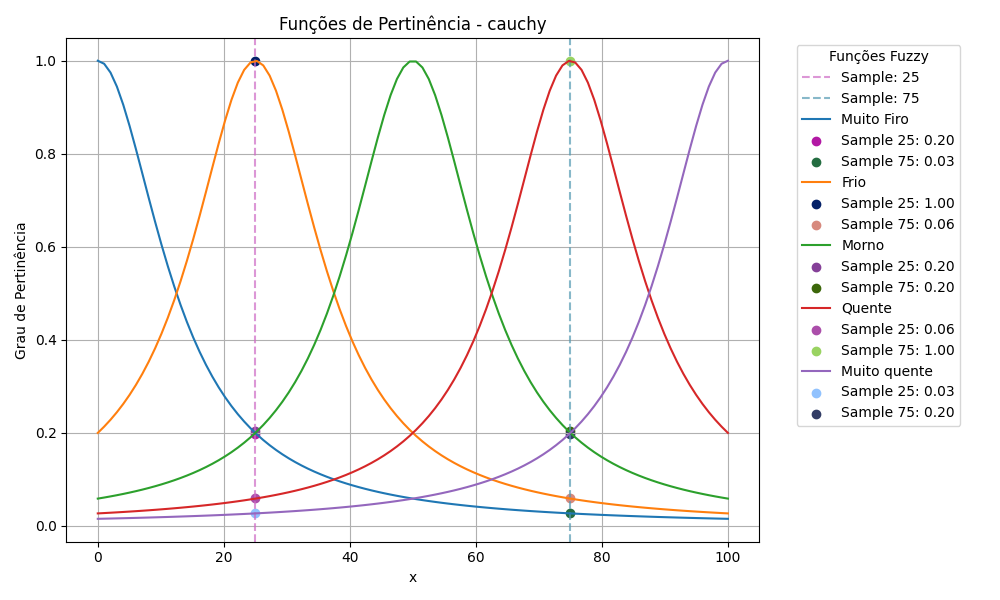
\includegraphics[width=0.8\textwidth]{img/funções_de_pertinência_cauchy_fuzzificado.png}
    \caption{Funções de Pertinência Cauchy para a variável \textbf{Temperatura}.}
\end{figure}

\subsubsection{Fuzzificação com Funções Double Gaussian}

Para a variável linguística \textbf{Temperatura}, foram definidos cinco conjuntos fuzzy com os seguintes intervalos e parâmetros, além das ativações calculadas para as amostras \textbf{25} e \textbf{75}:

\begin{table}[H]
\centering
\caption{Conjuntos Fuzzy, Intervalos, Parâmetros e Ativações (Double Gaussian)}
\begin{tabular}{|c|c|c|c|}
\hline
\textbf{Categoria}    & \textbf{Intervalo (°C)} & \textbf{Parâmetros}               & \textbf{Ativações [25, 75]} \\ \hline
Muita Fria            & $[0.0, 20.0]$          & $[0.0, 6.25, 12.5, 6.25]$         & $[0.12, 0.0]$              \\ \hline
Fria                  & $[20.0, 40.0]$         & $[12.5, 6.25, 37.5, 6.25]$        & $[0.15, 0.0]$              \\ \hline
Morno                 & $[40.0, 60.0]$         & $[37.5, 6.25, 62.5, 6.25]$        & $[0.15, 0.15]$             \\ \hline
Quente                & $[60.0, 80.0]$         & $[62.5, 6.25, 87.5, 6.25]$        & $[0.0, 0.15]$              \\ \hline
Muito Quente          & $[80.0, 100.0]$        & $[87.5, 6.25, 100.0, 6.25]$       & $[0.0, 0.12]$              \\ \hline
\end{tabular}
\end{table}

A seguir, apresentamos o gráfico das funções de pertinência Double Gaussian e suas ativações:

\begin{figure}[H]
    \centering
    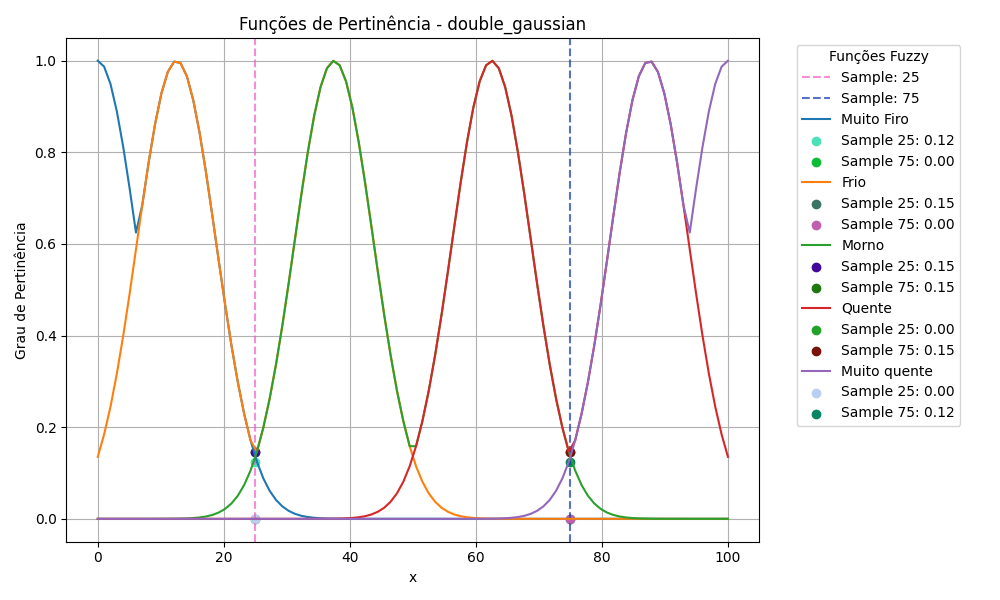
\includegraphics[width=0.8\textwidth]{img/funções_de_pertinência_double_gaussian_fuzzificado.png}
    \caption{Funções de Pertinência Double Gaussian para a variável \textbf{Temperatura}.}
\end{figure}

\subsubsection{Fuzzificação com Funções Logarítmicas}

Para a variável linguística \textbf{Temperatura}, foram definidos cinco conjuntos fuzzy com os seguintes intervalos e parâmetros, além das ativações calculadas para as amostras \textbf{25} e \textbf{75}:

\begin{table}[H]
\centering
\caption{Conjuntos Fuzzy, Intervalos, Parâmetros e Ativações (Logarítmica)}
\begin{tabular}{|c|c|c|c|}
\hline
\textbf{Categoria}    & \textbf{Intervalo (°C)} & \textbf{Parâmetros}       & \textbf{Ativações [25, 75]} \\ \hline
Muita Fria            & $[0.0, 20.0]$          & $[2.0, 1.0]$              & $[1, 1]$                   \\ \hline
Fria                  & $[20.0, 40.0]$         & $[2.0, 1.0]$              & $[1, 1]$                   \\ \hline
Morno                 & $[40.0, 60.0]$         & $[2.0, 1.0]$              & $[1, 1]$                   \\ \hline
Quente                & $[60.0, 80.0]$         & $[2.0, 1.0]$              & $[1, 1]$                   \\ \hline
Muito Quente          & $[80.0, 100.0]$        & $[2.0, 1.0]$              & $[1, 1]$                   \\ \hline
\end{tabular}
\end{table}

A seguir, apresentamos o gráfico das funções de pertinência Logarítmicas e suas ativações:

\begin{figure}[H]
    \centering
    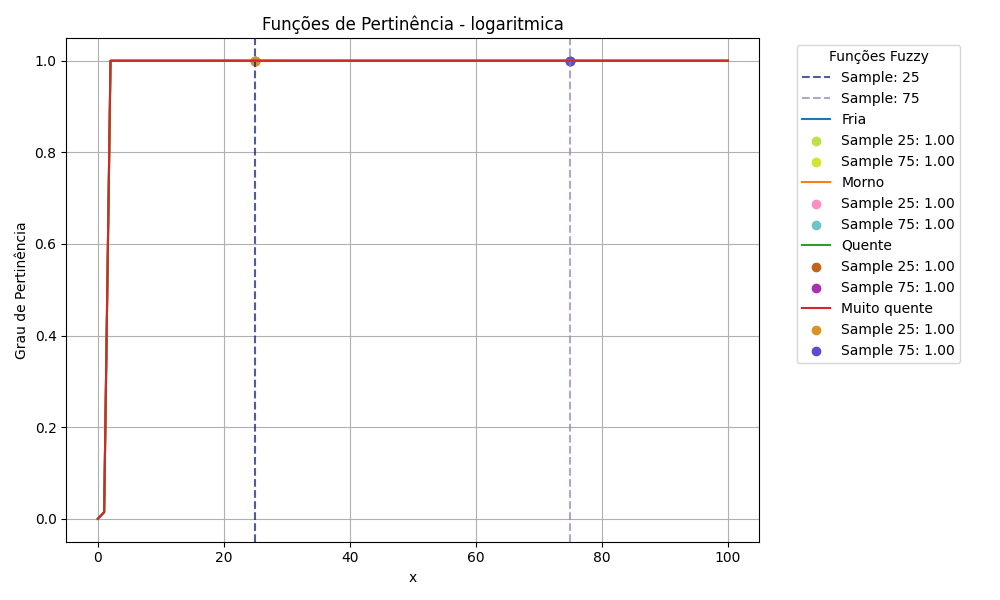
\includegraphics[width=0.8\textwidth]{img/funções_de_pertinência_logaritmica_fuzzificado.png}
    \caption{Funções de Pertinência Logarítmicas para a variável \textbf{Temperatura}.}
\end{figure}

\subsubsection{Fuzzificação com Funções Retangulares}

Para a variável linguística \textbf{Temperatura}, foram definidos cinco conjuntos fuzzy com os seguintes intervalos e parâmetros, além das ativações calculadas para as amostras \textbf{25} e \textbf{75}:

\begin{table}[H]
\centering
\caption{Conjuntos Fuzzy, Intervalos, Parâmetros e Ativações (Retangular)}
\begin{tabular}{|c|c|c|c|}
\hline
\textbf{Categoria}    & \textbf{Intervalo (°C)} & \textbf{Parâmetros}       & \textbf{Ativações [25, 75]} \\ \hline
Muita Fria            & $[0.0, 20.0]$          & $[0.0, 12.5]$             & $[0, 0]$                   \\ \hline
Fria                  & $[20.0, 40.0]$         & $[12.5, 37.5]$            & $[1, 0]$                   \\ \hline
Morno                 & $[40.0, 60.0]$         & $[37.5, 62.5]$            & $[0, 0]$                   \\ \hline
Quente                & $[60.0, 80.0]$         & $[62.5, 87.5]$            & $[0, 1]$                   \\ \hline
Muito Quente          & $[80.0, 100.0]$        & $[87.5, 100.0]$           & $[0, 0]$                   \\ \hline
\end{tabular}
\end{table}

A seguir, apresentamos o gráfico das funções de pertinência Retangulares e suas ativações:

\begin{figure}[H]
    \centering
    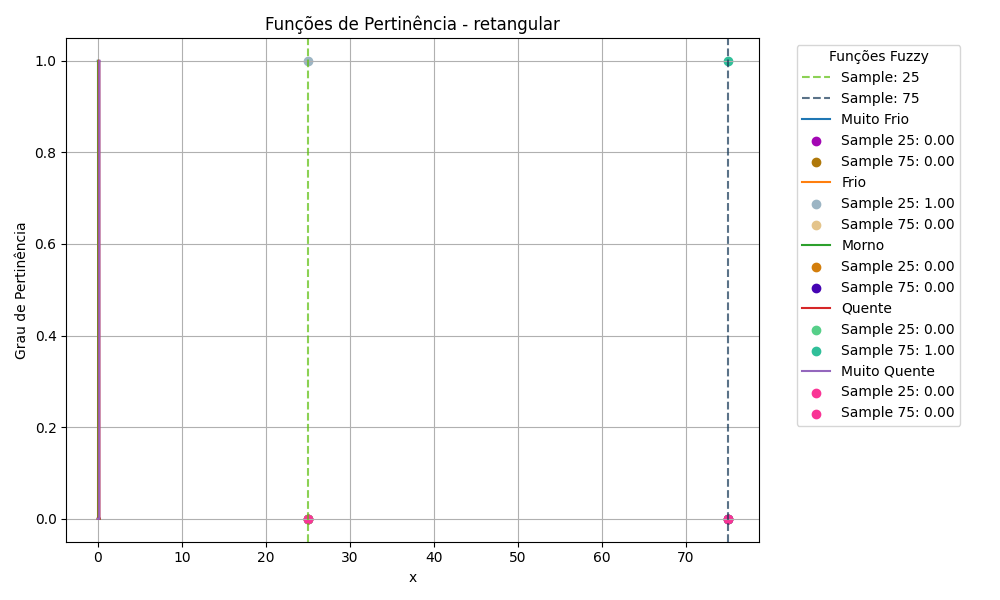
\includegraphics[width=0.8\textwidth]{img/funções_de_pertinência_retangular_fuzzificado.png}
    \caption{Funções de Pertinência Retangulares para a variável \textbf{Temperatura}.}
\end{figure}



\subsection{Conclusão}
Nesta seção, analisamos os resultados obtidos para as diferentes funções de pertinência aplicadas à variável linguística \textbf{Temperatura}. A análise considera como o grau de ativação varia entre as funções e identifica quais apresentam maior suavidade ou sensibilidade às variações no domínio.
Os resultados mostram que o grau de ativação varia de forma distinta entre as funções de pertinência:

\begin{itemize}
    \item \textbf{Funções Gaussianas}: Apresentam transições suaves e contínuas, com ativação máxima (1.0) para as categorias \textit{Fria} e \textit{Quente} nas amostras 25 e 75, respectivamente. As categorias adjacentes (\textit{Muita Fria} e \textit{Morno}) exibem ativações moderadas (0.13 e 0.14), indicando boa sensibilidade às variações no domínio.

    \item \textbf{Funções Sigmoidais}: Demonstram transições suaves e assimétricas. A categoria \textit{Muita Fria} apresenta ativação constante (1.0) para ambas as amostras, enquanto a categoria \textit{Fria} exibe uma ativação moderada (0.56) na amostra 25 e máxima (1.0) na amostra 75. As categorias \textit{Morno} e \textit{Quente} apresentam ativações crescentes, refletindo alta sensibilidade em torno dos pontos centrais.

    \item \textbf{Funções Bell}: Apresentam características semelhantes às gaussianas, mas com maior controle sobre a largura e inclinação. A categoria \textit{Fria} atinge ativação máxima (1.0) na amostra 25, enquanto as categorias adjacentes (\textit{Muita Fria} e \textit{Morno}) exibem ativações moderadas (0.06). Na amostra 75, a categoria \textit{Quente} apresenta ativação máxima (1.0), enquanto as categorias adjacentes exibem ativações baixas.

    \item \textbf{Funções S}: Apresentam transições suaves e crescentes. A categoria \textit{Muita Fria} exibe ativação constante (1.0) para ambas as amostras, enquanto a categoria \textit{Fria} apresenta ativação máxima (1.0) na amostra 75. A categoria \textit{Morno} exibe a maior ativação (1.96) na amostra 75, indicando alta sensibilidade em regiões de transição.

    \item \textbf{Funções Z}: Apresentam transições suaves e decrescentes. A categoria \textit{Morno} exibe ativação máxima (1.0) na amostra 25, enquanto a categoria \textit{Quente} apresenta ativação negativa (-0.96) na amostra 75, refletindo a natureza decrescente da função.

    \item \textbf{Funções Pi}: Combinam as características das funções S e Z, apresentando transições suaves em ambas as extremidades. A categoria \textit{Fria} exibe ativação máxima (1.0) na amostra 25, enquanto a categoria \textit{Quente} apresenta ativação elevada (1.96) na amostra 75.

    \item \textbf{Funções Singleton}: Apresentam ativações discretas, com valores nulos para todas as categorias e amostras. Isso reflete a ausência de transições, sendo adequadas apenas para modelar pontos específicos no domínio.

    \item \textbf{Funções Cauchy}: Apresentam transições suaves, com caudas mais longas em comparação às gaussianas. A categoria \textit{Fria} exibe ativação máxima (1.0) na amostra 25, enquanto as categorias adjacentes (\textit{Muita Fria} e \textit{Morno}) apresentam ativações moderadas (0.2). Na amostra 75, a categoria \textit{Quente} exibe ativação máxima (1.0).

    \item \textbf{Funções Double Gaussian}: Apresentam duas regiões de ativação controladas por parâmetros independentes. As categorias \textit{Fria} e \textit{Morno} exibem ativações moderadas (0.15) na amostra 25, enquanto a categoria \textit{Quente} apresenta ativação moderada (0.15) na amostra 75.

    \item \textbf{Funções Logarítmicas}: Apresentam ativações constantes (1.0) para todas as categorias e amostras, indicando baixa sensibilidade às variações no domínio.

    \item \textbf{Funções Retangulares}: Apresentam regiões planas com ativação constante (1.0) e transições abruptas nas bordas. A categoria \textit{Fria} exibe ativação máxima (1.0) na amostra 25, enquanto a categoria \textit{Quente} apresenta ativação máxima (1.0) na amostra 75.
\end{itemize}

A suavidade e a sensibilidade às variações no domínio variam significativamente entre as funções:

\begin{itemize}
    \item \textbf{Maior Suavidade}: As funções Gaussianas, Sigmoidais, Bell e Cauchy apresentam as transições mais suaves, sendo ideais para modelar mudanças graduais no grau de ativação.
    \item \textbf{Maior Sensibilidade}: As funções S e Pi demonstram alta sensibilidade em regiões de transição, enquanto as funções Gaussianas e Sigmoidais apresentam sensibilidade moderada.
    \item \textbf{Menor Suavidade e Sensibilidade}: As funções Retangulares e Singleton apresentam transições abruptas ou ausência de transição, sendo menos adequadas para modelar mudanças contínuas.
\end{itemize}

Os resultados mostram que as funções Gaussianas, Sigmoidais, Bell e Cauchy são as mais adequadas para modelar transições suaves e graduais. As funções S e Pi são úteis em cenários que exigem alta sensibilidade em regiões de transição. Por outro lado, as funções Retangulares e Singleton são mais indicadas para modelar intervalos bem definidos ou pontos discretos. A escolha da função de pertinência ideal depende do contexto da aplicação e das características desejadas para o sistema fuzzy.


\section{Operações Fuzzy}

As operações fuzzy são fundamentais para manipular conjuntos fuzzy e modelar incertezas em sistemas baseados em lógica fuzzy. Elas incluem complemento, união (t-conormas) e interseção (t-normas), permitindo combinar ou modificar graus de pertinência. Essas operações são amplamente utilizadas em aplicações práticas, como controle fuzzy, tomada de decisão e sistemas especialistas.

\subsection{Complemento, União e Interseção}

A lógica fuzzy estende a lógica clássica, permitindo lidar com incertezas ao atribuir graus de pertinência contínuos no intervalo $[0, 1]$. Agora vamos explora operações fuzzy fundamentais, como complemento (Zadeh, Sugeno, Yager), união (máximo, soma probabilística, soma limitada, soma drástica) e interseção (mínimo, produto, produto limitado, produto drástico). Utilizamos conjuntos fuzzy definidos por funções de pertinência (triangular, trapezoidal, gaussiana, etc.) para realizar análises gráficas e textuais comparativas, destacando as características e aplicações práticas de cada operador.



\subsubsection{Complemento}

As operações de complemento são utilizadas para calcular o grau de não-pertinência de um elemento a um conjunto fuzzy. Abaixo, apresentamos as fórmulas para os operadores de complemento Zadeh, Sugeno e Yager.


\paragraph{Operador Zadeh}

O complemento de Zadeh é definido como:
\[
\mu_{\text{Zadeh}}(x) = 1 - \mu(x)
\]

Os resultados para o operador de complemento Zadeh aplicado às funções de pertinência triangulares são apresentados na tabela abaixo. As ativações foram calculadas para as amostras \textbf{25} e \textbf{75}.

\begin{table}[H]
\centering
\caption{Ativações para o Operador Zadeh com Funções Triangulares}
\begin{tabular}{|c|c|c|c|}
\hline
\textbf{Categoria}    & \textbf{Intervalo (°C)} & \textbf{Parâmetros}       & \textbf{Ativações [25, 75]} \\ \hline
Muita Fria            & $[0.0, 20.0]$          & $[0.0, 0.0, 25.0]$        & $[1.0, 1.0]$               \\ \hline
Fria                  & $[20.0, 40.0]$         & $[0.0, 25.0, 50.0]$       & $[0.01, 1.0]$              \\ \hline
Morno                 & $[40.0, 60.0]$         & $[25.0, 50.0, 75.0]$      & $[0.99, 0.99]$             \\ \hline
Quente                & $[60.0, 80.0]$         & $[50.0, 75.0, 100.0]$     & $[1.0, 0.01]$              \\ \hline
Muito Quente          & $[80.0, 100.0]$        & $[75.0, 100.0, 100.0]$    & $[1.0, 1.0]$               \\ \hline
\end{tabular}
\end{table}

A figura abaixo apresenta o gráfico das funções de pertinência triangulares e seus complementos calculados utilizando o operador de Zadeh.

\begin{figure}[H]
    \centering
    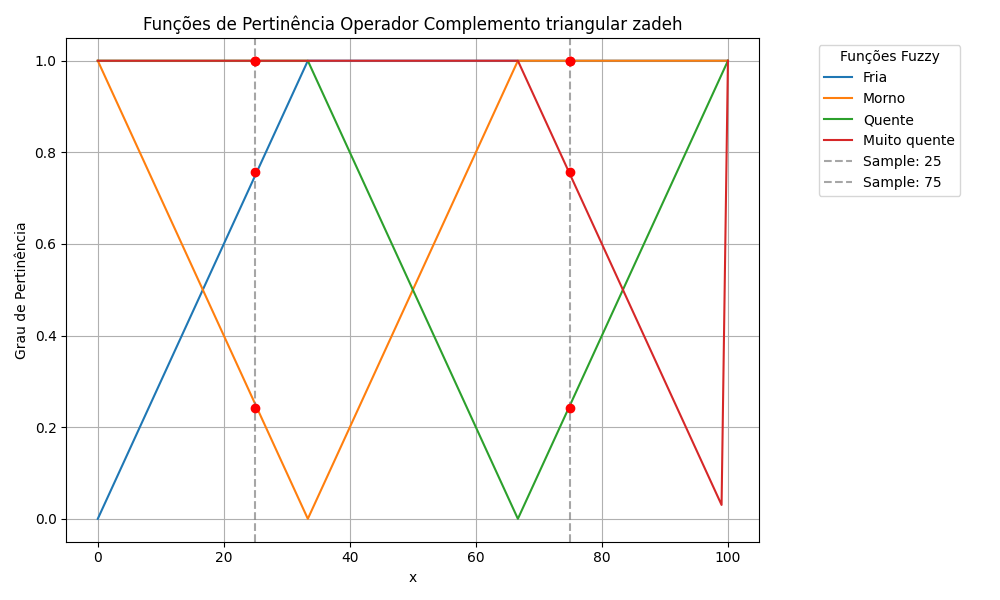
\includegraphics[width=0.8\textwidth]{img/funções_de_pertinência_operador_complemento_triangular_zadeh_fuzzificado.png}
    \caption{Funções de pertinência triangulares e seus complementos (Zadeh).}
    \label{fig:complemento_zadeh_triangular}
\end{figure}
Os resultados das ativações para os operadores de complemento Sugeno e Yager aplicados às funções de pertinência triangulares são apresentados nas tabelas abaixo. As ativações foram calculadas para as amostras \textbf{25} e \textbf{75}.

\paragraph{Operador Sugeno}

O complemento de Sugeno é definido como:
\[
\mu_{\text{Sugeno}}(x) = \frac{1 - \mu(x)}{1 + \lambda \cdot \mu(x)}
\]
onde $\lambda \geq 0$ é um parâmetro que controla a suavidade do complemento.
\begin{table}[H]
\centering
\caption{Ativações para o Operador Sugeno com Funções Triangulares}
\begin{tabular}{|c|c|c|c|}
\hline
\textbf{Categoria}    & \textbf{Intervalo (°C)} & \textbf{Parâmetros}       & \textbf{Ativações [25, 75]} \\ \hline
Muita Fria            & $[0.0, 20.0]$          & $[0.0, 0.0, 25.0]$        & $[1.0, 1.0]$               \\ \hline
Fria                  & $[20.0, 40.0]$         & $[0.0, 25.0, 50.0]$       & $[0.01, 1.0]$              \\ \hline
Morno                 & $[40.0, 60.0]$         & $[25.0, 50.0, 75.0]$      & $[0.98, 0.98]$             \\ \hline
Quente                & $[60.0, 80.0]$         & $[50.0, 75.0, 100.0]$     & $[1.0, 0.01]$              \\ \hline
Muito Quente          & $[80.0, 100.0]$        & $[75.0, 100.0, 100.0]$    & $[1.0, 1.0]$               \\ \hline
\end{tabular}
\end{table}

\begin{figure}[H]
    \centering
    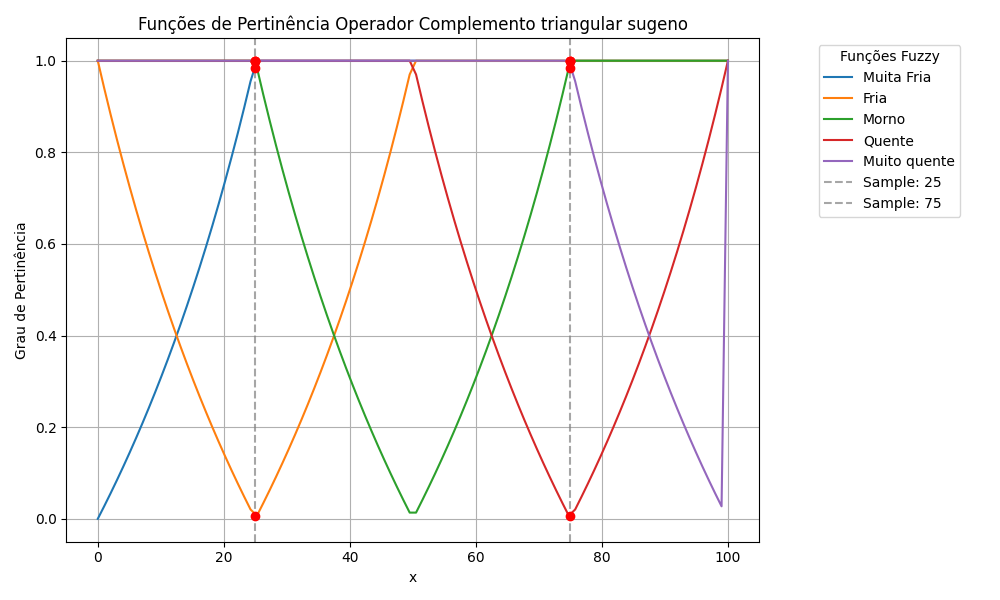
\includegraphics[width=0.8\textwidth]{img/funções_de_pertinência_operador_complemento_triangular_sugeno_fuzzificado.png}
    \caption{Funções de pertinência triangulares e seus complementos (Sugeno).}
    \label{fig:complemento_sugeno_triangular}
\end{figure}

\paragraph{Operador Yager}

O complemento de Yager é definido como:
\[
\mu_{\text{Yager}}(x) = \left(1 - \mu(x)^w\right)^{\frac{1}{w}}
\]
onde $w > 0$ é um parâmetro que ajusta a forma do complemento.

\begin{table}[H]
\centering
\caption{Ativações para o Operador Yager com Funções Triangulares}
\begin{tabular}{|c|c|c|c|}
\hline
\textbf{Categoria}    & \textbf{Intervalo (°C)} & \textbf{Parâmetros}       & \textbf{Ativações [25, 75]} \\ \hline
Muita Fria            & $[0.0, 20.0]$          & $[0.0, 0.0, 25.0]$        & $[1.0, 1.0]$               \\ \hline
Fria                  & $[20.0, 40.0]$         & $[0.0, 25.0, 50.0]$       & $[0.14, 1.0]$              \\ \hline
Morno                 & $[40.0, 60.0]$         & $[25.0, 50.0, 75.0]$      & $[1.0, 1.0]$               \\ \hline
Quente                & $[60.0, 80.0]$         & $[50.0, 75.0, 100.0]$     & $[1.0, 0.14]$              \\ \hline
Muito Quente          & $[80.0, 100.0]$        & $[75.0, 100.0, 100.0]$    & $[1.0, 1.0]$               \\ \hline
\end{tabular}
\end{table}

\begin{figure}[H]
    \centering
    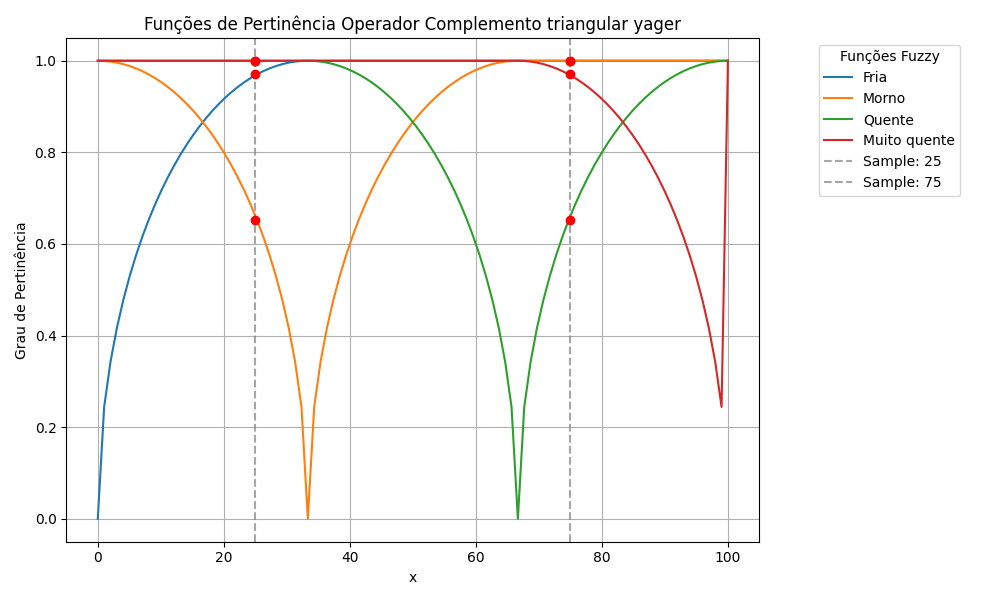
\includegraphics[width=0.8\textwidth]{img/funções_de_pertinência_operador_complemento_triangular_yager_fuzzificado.png}
    \caption{Funções de pertinência triangulares e seus complementos (Yager).}
    \label{fig:complemento_yager_triangular}
\end{figure}

\subsection{União (t-conormas)}

Os resultados das ativações para os operadores de união (t-conormas) aplicados às funções de pertinência triangulares são apresentados nas tabelas abaixo. As ativações foram calculadas para as amostras \textbf{25} e \textbf{75}.

\paragraph{Operador Máximo}

A união pelo operador máximo é definida como:
\[
\mu_{\text{Máximo}}(x) = \max(\mu_1(x), \mu_2(x))
\]

\begin{table}[H]
\centering
\caption{Ativações para o Operador Máximo com Funções Triangulares}
\begin{tabular}{|c|c|c|c|}
\hline
\textbf{Categoria}    & \textbf{Intervalo (°C)} & \textbf{Parâmetros}       & \textbf{Ativações [25, 75]} \\ \hline
Fria                  & $[0.0, 25.0]$          & $[0.0, 0.0, 33.33]$       & $[0.24, 0.0]$              \\ \hline
Morno                 & $[25.0, 50.0]$         & $[0.0, 33.33, 66.67]$     & $[0.76, 0.0]$              \\ \hline
Quente                & $[50.0, 75.0]$         & $[33.33, 66.67, 100.0]$   & $[0.0, 0.76]$              \\ \hline
Muito Quente          & $[75.0, 100.0]$        & $[66.67, 100.0, 100.0]$   & $[0.0, 0.24]$              \\ \hline
\textbf{Máximo} & -                     & -                         & $[0.76, 0.0]$             \\ \hline
\end{tabular}
\end{table}

\begin{figure}[H]
    \centering
    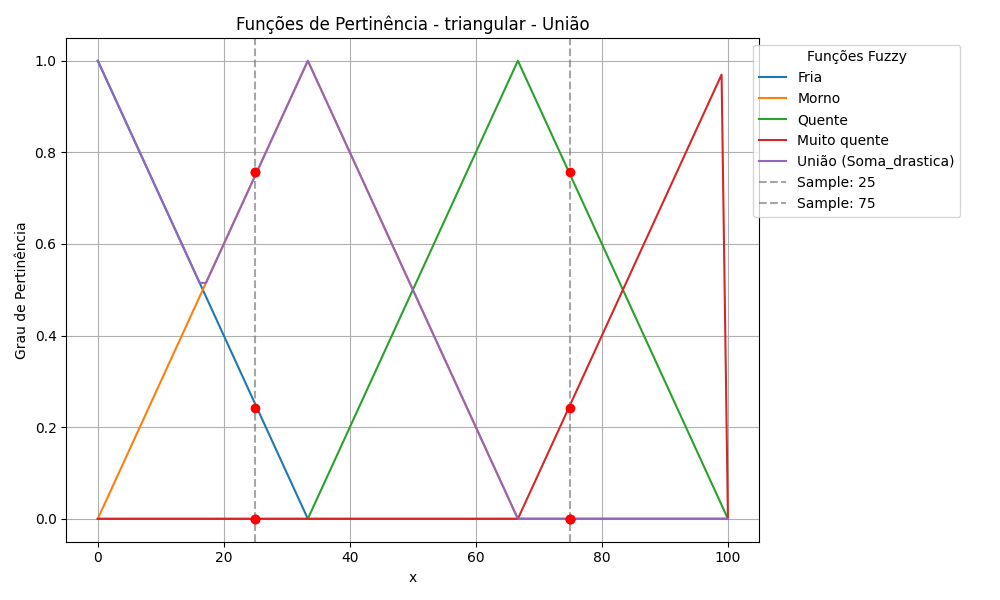
\includegraphics[width=0.8\textwidth]{img/funções_de_pertinência_triangular_união_fuzzificado.png}
    \caption{Funções de pertinência triangulares e suas uniões (Máximo).}
    \label{fig:uniao_maximo_triangular}
\end{figure}

\paragraph{Operador Soma Probabilística}

A união pelo operador soma probabilística é definida como:
\[
\mu_{\text{Soma Probabilística}}(x) = \mu_1(x) + \mu_2(x) - \mu_1(x) \cdot \mu_2(x)
\]

\begin{table}[H]
\centering
\caption{Ativações para o Operador Soma Probabilística com Funções Triangulares}
\begin{tabular}{|c|c|c|c|}
\hline
\textbf{Categoria}    & \textbf{Intervalo (°C)} & \textbf{Parâmetros}       & \textbf{Ativações [25, 75]} \\ \hline
Fria                  & $[0.0, 25.0]$          & $[0.0, 0.0, 33.33]$       & $[0.24, 0.0]$              \\ \hline
Morno                 & $[25.0, 50.0]$         & $[0.0, 33.33, 66.67]$     & $[0.76, 0.0]$              \\ \hline
Quente                & $[50.0, 75.0]$         & $[33.33, 66.67, 100.0]$   & $[0.0, 0.76]$              \\ \hline
Muito Quente          & $[75.0, 100.0]$        & $[66.67, 100.0, 100.0]$   & $[0.0, 0.24]$              \\ \hline
\textbf{Soma Probabilística} & -       & -                         & $[0.82, 0.0]$             \\ \hline
\end{tabular}
\end{table}

\paragraph{Operador Soma Limitada}

A união pelo operador soma limitada é definida como:
\[
\mu_{\text{Soma Limitada}}(x) = \min(1, \mu_1(x) + \mu_2(x))
\]

\begin{table}[H]
\centering
\caption{Ativações para o Operador Soma Limitada com Funções Triangulares}
\begin{tabular}{|c|c|c|c|}
\hline
\textbf{Categoria}    & \textbf{Intervalo (°C)} & \textbf{Parâmetros}       & \textbf{Ativações [25, 75]} \\ \hline
Fria                  & $[0.0, 25.0]$          & $[0.0, 0.0, 33.33]$       & $[0.24, 0.0]$              \\ \hline
Morno                 & $[25.0, 50.0]$         & $[0.0, 33.33, 66.67]$     & $[0.76, 0.0]$              \\ \hline
Quente                & $[50.0, 75.0]$         & $[33.33, 66.67, 100.0]$   & $[0.0, 0.76]$              \\ \hline
Muito Quente          & $[75.0, 100.0]$        & $[66.67, 100.0, 100.0]$   & $[0.0, 0.24]$              \\ \hline
\textbf{Soma Limitada} & -            & -                         & $[1.0, 0.0]$             \\ \hline
\end{tabular}
\end{table}

\begin{figure}[H]
    \centering
    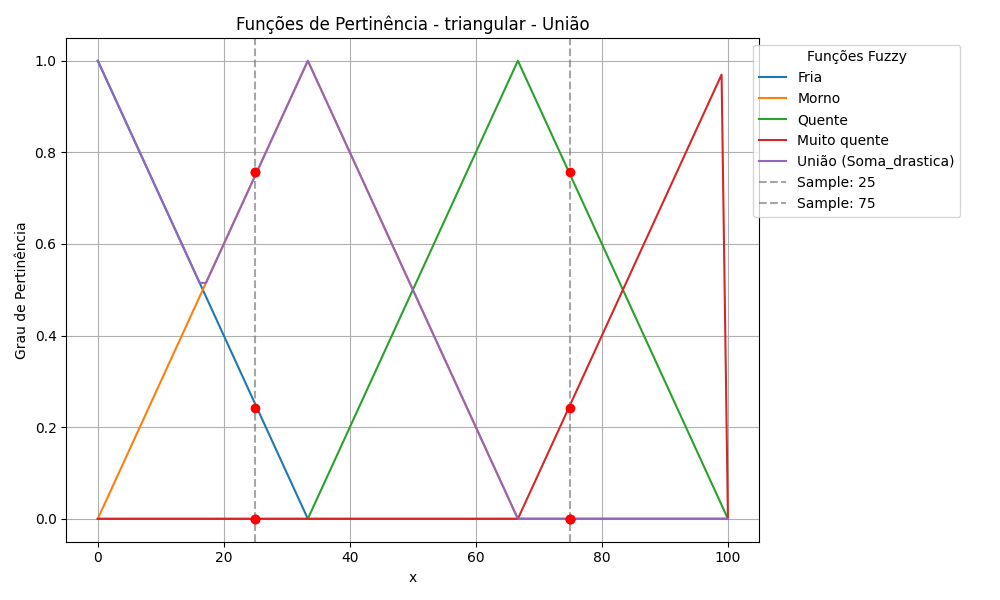
\includegraphics[width=0.8\textwidth]{img/funções_de_pertinência_triangular_união_fuzzificado.png}
    \caption{Funções de pertinência triangulares e suas uniões (Soma Limitada).}
    \label{fig:uniao_soma_limitada_triangular}
\end{figure}

\paragraph{Operador Soma Drástica}

A união pelo operador soma drástica é definida como:
\[
\mu_{\text{Soma Drástica}}(x) =
\begin{cases}
\max(\mu_1(x), \mu_2(x)), & \text{se } \min(\mu_1(x), \mu_2(x)) > 0, \\
0, & \text{caso contrário.}
\end{cases}
\]

\begin{table}[H]
\centering
\caption{Ativações para o Operador União (Soma Drástica) com Funções Triangulares}
\begin{tabular}{|c|c|c|c|}
\hline
\textbf{Categoria}    & \textbf{Intervalo (°C)} & \textbf{Parâmetros}       & \textbf{Ativações [25, 75]} \\ \hline
Fria                  & $[0.0, 25.0]$          & $[0.0, 0.0, 33.33]$       & $[0.24, 0.0]$              \\ \hline
Morno                 & $[25.0, 50.0]$         & $[0.0, 33.33, 66.67]$     & $[0.76, 0.0]$              \\ \hline
Quente                & $[50.0, 75.0]$         & $[33.33, 66.67, 100.0]$   & $[0.0, 0.76]$              \\ \hline
Muito Quente          & $[75.0, 100.0]$        & $[66.67, 100.0, 100.0]$   & $[0.0, 0.24]$              \\ \hline
\textbf{Soma Drástica} & -            & -                         & $[0.76, 0.0]$             \\ \hline
\end{tabular}
\end{table}

\begin{figure}[H]
    \centering
    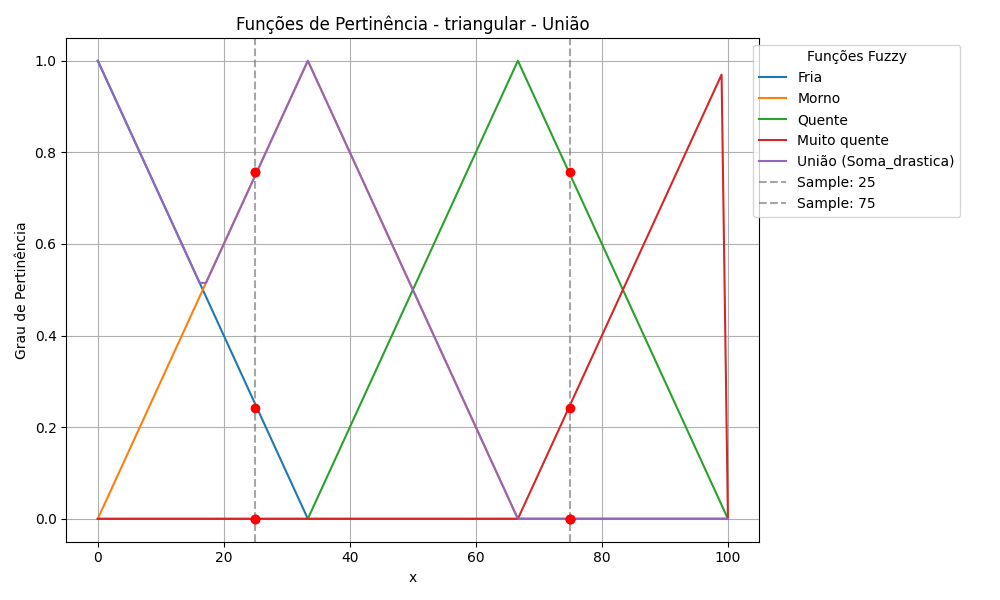
\includegraphics[width=0.8\textwidth]{img/funções_de_pertinência_triangular_união_fuzzificado.png}
    \caption{Funções de pertinência triangulares e suas uniões (Soma Drástica).}
    \label{fig:uniao_soma_drastica_triangular}
\end{figure}

\subsection{Intersecão (t-normas):}

\paragraph{Operador Produto Drástico}

A interseção pelo operador produto drástico é definida como:
\[
\mu_{\text{Produto Drástico}}(x) =
\begin{cases}
\max(\mu_1(x), \mu_2(x)), & \text{se } \min(\mu_1(x), \mu_2(x)) > 0, \\
0, & \text{caso contrário.}
\end{cases}
\]

\begin{table}[H]
\centering
\caption{Ativações para o Operador Produto Drástico com Funções Triangulares}
\begin{tabular}{|c|c|c|c|}
\hline
\textbf{Categoria}    & \textbf{Intervalo (°C)} & \textbf{Parâmetros}       & \textbf{Ativações [25, 75]} \\ \hline
Fria                  & $[0.0, 25.0]$          & $[0.0, 0.0, 33.33]$       & $[0.24, 0.0]$              \\ \hline
Morno                 & $[25.0, 50.0]$         & $[0.0, 33.33, 66.67]$     & $[0.76, 0.0]$              \\ \hline
Quente                & $[50.0, 75.0]$         & $[33.33, 66.67, 100.0]$   & $[0.0, 0.76]$              \\ \hline
Muito Quente          & $[75.0, 100.0]$        & $[66.67, 100.0, 100.0]$   & $[0.0, 0.24]$              \\ \hline
\textbf{Produto Drástico} & -     & -                         & $[0.0, 0.0]$              \\ \hline
\end{tabular}
\end{table}

\begin{figure}[H]
    \centering
    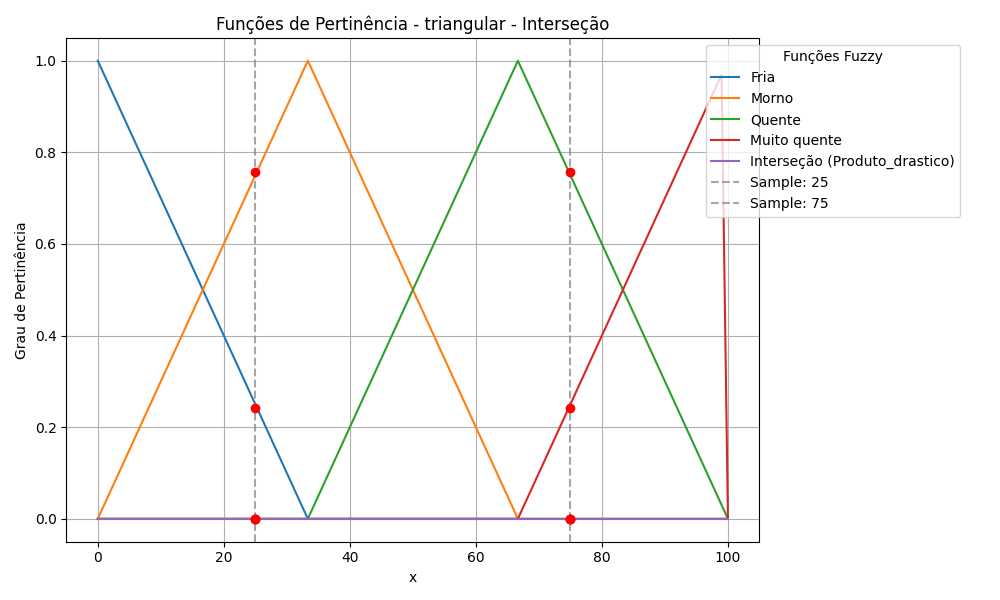
\includegraphics[width=0.8\textwidth]{img/funções_de_pertinência_triangular_interseção_fuzzificado.png}
    \caption{Funções de pertinência triangulares e suas interseções (Produto Drástico).}
    \label{fig:intersecao_produto_drastico_triangular}
\end{figure}

\paragraph{Operador Produto Drástico}

A interseção pelo operador produto drástico é definida como:
\[
\mu_{\text{Produto Drástico}}(x) =
\begin{cases}
\max(\mu_1(x), \mu_2(x)), & \text{se } \min(\mu_1(x), \mu_2(x)) > 0, \\
0, & \text{caso contrário.}
\end{cases}
\]

\begin{table}[H]
\centering
\caption{Ativações para o Operador Produto Drástico com Funções Triangulares}
\begin{tabular}{|c|c|c|c|}
\hline
\textbf{Categoria}    & \textbf{Intervalo (°C)} & \textbf{Parâmetros}       & \textbf{Ativações [25, 75]} \\ \hline
Fria                  & $[0.0, 25.0]$          & $[0.0, 0.0, 33.33]$       & $[0.24, 0.0]$              \\ \hline
Morno                 & $[25.0, 50.0]$         & $[0.0, 33.33, 66.67]$     & $[0.76, 0.0]$              \\ \hline
Quente                & $[50.0, 75.0]$         & $[33.33, 66.67, 100.0]$   & $[0.0, 0.76]$              \\ \hline
Muito Quente          & $[75.0, 100.0]$        & $[66.67, 100.0, 100.0]$   & $[0.0, 0.24]$              \\ \hline
\textbf{Produto Drástico} & -     & -                         & $[0.0, 0.0]$              \\ \hline
\end{tabular}
\end{table}

\begin{figure}[H]
    \centering
    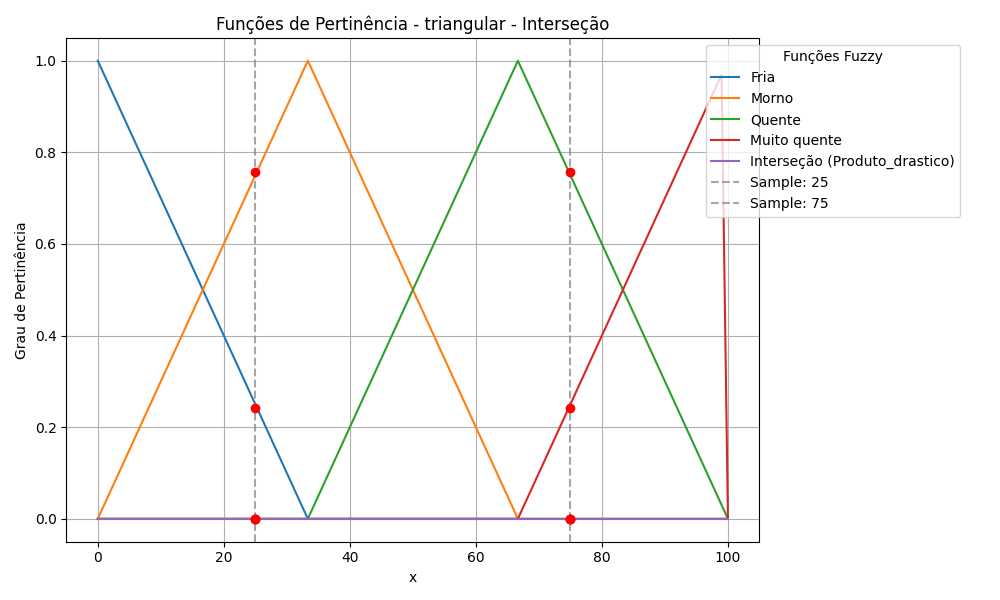
\includegraphics[width=0.8\textwidth]{img/funções_de_pertinência_triangular_interseção_fuzzificado.png}
    \caption{Funções de pertinência triangulares e suas interseções (Produto Drástico).}
    \label{fig:intersecao_produto_drastico_triangular}
\end{figure}
\subsubsection{Conclusão}

Os operadores de complemento analisados apresentam características distintas que os tornam adequados para diferentes aplicações:

\begin{itemize}
    \item \textbf{Zadeh}: Simples e direto, ideal para aplicações gerais onde não há necessidade de ajustes adicionais na suavidade do complemento.
    \item \textbf{Sugeno}: Permite ajuste de suavidade por meio do parâmetro $\lambda$, sendo mais flexível e adaptável a diferentes cenários.
    \item \textbf{Yager}: Oferece maior controle sobre a forma do complemento por meio do parâmetro $w$, sendo útil em cenários específicos que exigem maior personalização.
\end{itemize}

A escolha do operador de complemento deve considerar o contexto da aplicação e os requisitos específicos do sistema fuzzy.

\subsection{Relação Fuzzy}

Neste exemplo, consideramos dois conjuntos fuzzy representando categorias de \textit{Temperatura} (\textit{Fria}, \textit{Morna}, \textit{Quente}, \textit{Muito Quente}) e \textit{Umidade} (\textit{Baixa}, \textit{Moderada}, \textit{Alta}, \textit{Muito Alta}). Os graus de pertinência para cada categoria são definidos como:

\begin{itemize}
    \item Conjunto A (\textit{Temperatura}): $[0.1, 0.5, 0.8, 1.0]$
    \item Conjunto B (\textit{Umidade}): $[0.2, 0.4, 0.7, 0.9]$
\end{itemize}

Utilizamos diferentes operadores t-norma e s-norma para calcular as matrizes de relação fuzzy entre os conjuntos, destacando as interações entre os graus de pertinência.

\subsubsection{t-Norma (Mínimo)}

\textbf{t-Norma (Mínimo)}:
\[
\mu_{\text{Mínimo}}(x, y) = \min(\mu_A(x), \mu_B(y))
\]

\[
R_{\text{Mínimo}} =
\begin{bmatrix}
0.1 & 0.1 & 0.1 & 0.1 \\
0.2 & 0.4 & 0.5 & 0.5 \\
0.2 & 0.4 & 0.7 & 0.8 \\
0.2 & 0.4 & 0.7 & 0.9
\end{bmatrix}
\]

\subsubsection{t-Norma (Produto)}

\textbf{t-Norma (Produto)}:
\[
\mu_{\text{Produto}}(x, y) = \mu_A(x) \cdot \mu_B(y)
\]

\[
R_{\text{Produto}} =
\begin{bmatrix}
0.02 & 0.04 & 0.07 & 0.09 \\
0.10 & 0.20 & 0.35 & 0.45 \\
0.16 & 0.32 & 0.56 & 0.72 \\
0.20 & 0.40 & 0.70 & 0.90
\end{bmatrix}
\]

\subsubsection{s-Norma (Máximo)}

\textbf{s-Norma (Máximo)}:
\[
\mu_{\text{Máximo}}(x, y) = \max(\mu_A(x), \mu_B(y))
\]

\[
R_{\text{Máximo}} =
\begin{bmatrix}
0.2 & 0.4 & 0.7 & 0.9 \\
0.5 & 0.5 & 0.7 & 0.9 \\
0.8 & 0.8 & 0.8 & 0.9 \\
1.0 & 1.0 & 1.0 & 1.0
\end{bmatrix}
\]

\subsubsection{s-Norma (Soma Probabilística)}

\textbf{s-Norma (Soma Probabilística)}:
\[
\mu_{\text{Soma Probabilística}}(x, y) = \mu_A(x) + \mu_B(y) - \mu_A(x) \cdot \mu_B(y)
\]

\[
R_{\text{Soma Probabilística}} =
\begin{bmatrix}
0.28 & 0.46 & 0.73 & 0.91 \\
0.60 & 0.70 & 0.85 & 0.95 \\
0.84 & 0.88 & 0.94 & 0.98 \\
1.00 & 1.00 & 1.00 & 1.00
\end{bmatrix}
\]

\subsubsection{Conclusão}

A seguir, destacamos as principais características de cada operador com base nos resultados obtidos:

\begin{itemize}
    \item \textbf{t-Norma (Mínimo)}:
    \begin{itemize}
        \item Este operador reflete a interseção mais conservadora entre os conjuntos fuzzy.
        \item A matriz resultante apresenta valores que representam o menor grau de pertinência entre os elementos dos conjuntos.
        \item É útil em aplicações onde se deseja garantir que a relação fuzzy seja restritiva e conservadora.
    \end{itemize}

    \item \textbf{t-Norma (Produto)}:
    \begin{itemize}
        \item Este operador permite suavização, gerando valores intermediários que refletem a interação proporcional entre os conjuntos fuzzy.
        \item A matriz resultante apresenta valores que são o produto dos graus de pertinência dos elementos.
        \item É ideal para modelar relações mais flexíveis e contínuas.
    \end{itemize}

    \item \textbf{s-Norma (Máximo)}:
    \begin{itemize}
        \item Este operador reflete a união mais abrangente entre os conjuntos fuzzy.
        \item A matriz resultante apresenta valores que representam o maior grau de pertinência entre os elementos dos conjuntos.
        \item É adequado para cenários onde se deseja destacar a união dos conjuntos.
    \end{itemize}

    \item \textbf{s-Norma (Soma Probabilística)}:
    \begin{itemize}
        \item Este operador reflete a união com suavização, garantindo que o resultado não ultrapasse 1.
        \item A matriz resultante apresenta valores que combinam os graus de pertinência dos elementos de forma probabilística.
        \item É útil em aplicações onde se deseja modelar interações suaves entre os conjuntos.
    \end{itemize}
\end{itemize}

Os operadores analisados apresentam comportamentos distintos que os tornam adequados para diferentes aplicações:

\begin{itemize}
    \item O \textbf{t-Norma (Mínimo)} é mais conservador e restritivo, sendo útil em cenários onde a precisão é essencial.
    \item O \textbf{t-Norma (Produto)} oferece uma abordagem mais suave e proporcional, sendo ideal para modelar interações contínuas.
    \item O \textbf{s-Norma (Máximo)} destaca a união dos conjuntos, sempre puxando para o maior grau de pertinência.
    \item O \textbf{s-Norma (Soma Probabilística)} combina suavidade e flexibilidade, sendo útil em aplicações que exigem modelagem probabilística.
\end{itemize}


\subsection{Composição de Relações Fuzzy}

Neste exemplo, consideramos dois conjuntos fuzzy representando categorias de \textit{Temperatura} (\textit{Fria}, \textit{Morna}, \textit{Quente}) e \textit{Umidade} (\textit{Baixa}, \textit{Moderada}, \textit{Alta}). As matrizes fuzzy foram calculadas utilizando diferentes operadores de composição.

\textbf{Matriz de Temperatura} (\textit{Fria, Morna, Quente}):
\[
\text{Temperatura} =
\begin{bmatrix}
0.1 & 0.5 & 0.8 \\
0.2 & 0.6 & 0.9 \\
0.3 & 0.7 & 1.0
\end{bmatrix}
\]

\textbf{Matriz de Umidade} (\textit{Baixa, Moderada, Alta}):
\[
\text{Umidade} =
\begin{bmatrix}
0.2 & 0.4 & 0.7 \\
0.3 & 0.5 & 0.8 \\
0.4 & 0.6 & 0.9
\end{bmatrix}
\]


As matrizes de composição fuzzy calculadas para os operadores acima são apresentadas a seguir:

\subsubsection{Máximo-Mínimo}
\textbf{Máximo-Mínimo}:
    \[
    \mu_R(x, z) = \max_y \min(\mu_A(x, y), \mu_B(y, z))
    \]

\[
R_{\text{Máximo-Mínimo}} =
\begin{bmatrix}
0.4 & 0.6 & 0.8 \\
0.4 & 0.6 & 0.9 \\
0.4 & 0.6 & 0.9
\end{bmatrix}
\]

\subsubsection{Mínimo-Máximo}

\textbf{Mínimo-Máximo}:
    \[
    \mu_R(x, z) = \min_y \max(\mu_A(x, y), \mu_B(y, z))
    \]
\[
R_{\text{Mínimo-Máximo}} =
\begin{bmatrix}
0.2 & 0.4 & 0.7 \\
0.2 & 0.4 & 0.7 \\
0.3 & 0.4 & 0.7
\end{bmatrix}
\]

\subsubsection{Máximo-Produto}

\textbf{Máximo-Produto}:
    \[
    \mu_R(x, z) = \max_y (\mu_A(x, y) \cdot \mu_B(y, z))
    \]

\[
R_{\text{Máximo-Produto}} =
\begin{bmatrix}
0.32 & 0.48 & 0.72 \\
0.36 & 0.54 & 0.81 \\
0.40 & 0.60 & 0.90
\end{bmatrix}
\]
\subsection{Conclusão}

A seguir, destacamos as principais características de cada operador com base nos resultados obtidos:

\begin{itemize}
    \item \textbf{Máximo-Mínimo}:
    \begin{itemize}
        \item Este operador reflete a interseção mais conservadora entre os conjuntos fuzzy.
        \item A matriz resultante apresenta valores que representam o maior grau de pertinência mínimo entre os elementos dos conjuntos.
        \item É útil em aplicações onde se deseja garantir que a relação fuzzy seja restritiva e conservadora.
    \end{itemize}

    \item \textbf{Mínimo-Máximo}:
    \begin{itemize}
        \item Este operador reflete a união mais conservadora entre os conjuntos fuzzy.
        \item A matriz resultante apresenta valores que representam o menor grau de pertinência máximo entre os elementos dos conjuntos.
        \item É adequado para cenários onde se deseja modelar relações menos restritivas, mas ainda conservadoras.
    \end{itemize}

\item \textbf{Máximo-Produto}:
    \begin{itemize}
        \item Este operador permite suavização, considerando o produto dos graus de pertinência.
        \item A matriz resultante apresenta valores intermediários, refletindo a interação proporcional entre os conjuntos fuzzy.
        \item É ideal para aplicações onde se deseja modelar relações mais flexíveis e contínuas.
    \end{itemize}
\end{itemize}

Os operadores analisados apresentam comportamentos distintos que os tornam adequados para diferentes aplicações:

\begin{itemize}
    \item O \textbf{Máximo-Mínimo} é mais conservador e restritivo, sendo útil em cenários onde a precisão é essencial.
    \item O \textbf{Mínimo-Máximo} oferece uma abordagem mais flexível, mas ainda conservadora, sendo adequado para modelar relações menos restritivas.
    \item O \textbf{Máximo-Produto} é o mais suave e flexível, permitindo modelar interações contínuas e graduais entre os conjuntos fuzzy.
\end{itemize}




\end{document}